\documentclass[a4paper, 11pt]{report}
\usepackage{preamble}

\begin{document}\maketitle

\tableofcontents

\chapter{Introduction}

\chapter{Background: The double flag variety approach to q-Schur algebras}

\section{Flag varieties as projective algebraic varieties}

{\color{blue}Include a discussion of flag varieties in a finite dimensional vector space. Explain: topology of projective space; Pl\"{u}cker embedding of Grassmannian in a projective space; flag varieties as a closed subset in a product of Grassmannians - show that the inclusion of one subspace into another is a closed condition - given by vanishing of some homogenous polynomials which should appear as minors of a matrix.}

References for this material include \cite{harris13}[J. Harris: A First Course in Algebraic Geometry]; \cite{hu07}[D. Hudec: The Grassmannian as a Projective Variety]; \cite{morandi98}[P. Morandi: Algebraic Groups, Grassmannians and Flag Varieties].

\chapter{The cyclic flags approach to affine q-Schur algebras}

Fix natural numbers $n$ and $r$.

\begin{definition}[compositions]\label{def:compositions}
A composition of $r$ into $n$ parts is an $n$-tuple $\lambda=(\lambda_1,\ldots,\lambda_n)\in\integers^n$ of non-negative integers whose sum equals $r$. Denote the set of compositions of $r$ into $n$ parts by $\compositions$.
\end{definition}

\begin{definition}[infinite periodic matrices]\label{def:matrices}
Let $\matrices$ be the set of matrices $A=(a_{i,j})_{i,j\in\integers}$ with integer entries $a_{i,j}$ satisfying the following conditions: 
\begin{itemize}
\item
$a_{i,j}\geq 0$ for each $i,j\in\integers$;
\item
each row or column has only finitely many non-zero entries;
\item
the sum of the entries in any $n$ consecutive rows or columns equals $r$;
\item
$a_{i-n,j-n}=a_{i,j}$ for each $i,j\in\integers$.
\end{itemize}
These matrices are referred to as infinite periodic matrices.
\end{definition}

\begin{definition}[source and target]\label{def:source-target}
Given $A\in\matrices$, let $\ro{A}$ and $\co{A}$ be the compositions of $r$ into $n$ parts given by
\begin{equation*}
\ro{A} = \left( \sum_{j\in\integers}a_{1,j}, \ldots, \sum_{j\in\integers} a_{n,j}\right)
\end{equation*}
and
\begin{equation*}
\co{A} = \left( \sum_{i\in\integers} a_{i,1}, \ldots, \sum_{i\in\integers} a_{i,n}\right).
\end{equation*}
$A\in\matrices$ is said to go from $\co{A}$ to $\ro{A}$.
\end{definition}

\begin{definition}[diagonal matrices]\label{def:diagonal-matrices}
Given $\lambda\in\compositions$, let $D_\lambda\in\matrices$ be the matrix given by $(D_\lambda)_{i,j}=0$ for $i,j\in\integers$ with $i\neq j$ and $(D_\lambda)_{i,i}=\lambda_i$ for $i\in\integers$; where the indices are taken modulo $n$.
\end{definition}

\section{Cyclic flags}

Fix $n,r\in\naturals$ and let $\field$ be a field. Let $\laurent$ be the $\field$-algebra $\field[\epsilon,\epsilon^{-1}]$ and let $\polys$ be the subalgebra generated by $\epsilon$, so $\polys = \field[\epsilon]$. Let $V$ be a free $\laurent$-module of rank $r$. Let $G$ be the automorphism group of the $\laurent$-module $V$, so $G$ is isomorphic to $\GL{r}{\laurent}$. A lattice in $V$ is a $\polys$-submodule $L$ of $V$ with $\laurent\otimes_\polys L = V$. In particular, a lattice is an $\polys$-submodule of $V$ which is a free $\polys$-module of rank $r$.

\begin{lemma}
Let $L$ be a lattice in $V$. $L/{\epsilon L}$ is a torsion $\polys$-module, where $\epsilon$ acts as zero. $L/{\epsilon L}$ is a free $\polys/{\langle \epsilon \rangle}$-module of rank $r$; that is, $L/{\epsilon L}$ is an $r$-dimensional $\field$-vector space.
\end{lemma}
\begin{proof}
$L$ is a free $\polys$-module of rank $r$, with $L\subset V$. Given an $\polys$-basis $\{x_1,\ldots,x_r\}$ of $L$, $\{\epsilon x_1,\ldots, \epsilon x_r\}$ is an $\polys$-basis of $\epsilon L$. Finally, the cosets $\{ x_1 + \epsilon L,\ldots, x_r + \epsilon L\}$ give a basis for $L/{\epsilon L}$ over $\polys/{\langle \epsilon\rangle}\cong \field$.
\end{proof}

Let $\flags=\flags_\field(n,r)$ be the set of collections $(L_i)_{i\in\integers}$ of lattices in $V$ with $L_i\subset L_{i+1}$ and $\epsilon L_i = L_{i-n}$ for each $i\in\integers$. These collections of lattices in $V$ are referred to as cyclic flags in $V$. 

$G$ acts on $\flags$ by $(g\cdot L)_i = g(L_i)$ for each $i\in\integers$, given $g\in G$ and $L\in\flags$. The $G$-orbits in $\flags$ are indexed by the set $\compositions$ of compositions of $r$ into $n$ parts: the $G$-orbit in $\flags$ corresponding to $\lambda\in\compositions$ is
\begin{equation*}
\flags_\lambda = \left\{L\in\flags: \dim\left(\frac{L_i}{L_{i-1}}\right) = \lambda_i \text{ for each } i\in\integers\right\}
\end{equation*}

\begin{definition}\label{def:characteristic-matrix}
The periodic characteristic matrix of a pair of cyclic flags $(L,L')\in\dblflags$ is the matrix $\type{L}{L'}=(a_{i,j})_{i,j\in\integers}$ with entries
\begin{equation*}
a_{i,j} = \dim_\field\left(\frac{L_i\cap L_j'}{L_i\cap L_{j-1}' + L_{i-1}\cap L_j'}\right)
\end{equation*}
for each $i,j\in\integers$.
\end{definition}

The diagonal action of $G$ on $\dblflags$ has orbits indexed by the set $\matrices$ of infinite periodic matrices (see definition \ref{def:matrices}). The $G$-orbit corresponding to $A\in\matrices$ is denoted $\orbit{A}$ and consists of those pairs $(L,L')\in\dblflags$ with periodic characteristic matrix $\type{L}{L'}$ equal to $A$.

\begin{lemma}(alternative expression for characteristic matrix)
Alternatively,
\begin{equation*}
a_{i,j} = \dim_\field\left(\frac{L_{i-1} + L_i\cap L_j'}{L_{i-1} + L_i\cap L_{j-1}'}\right)
\end{equation*}
for each $i,j\in\integers$.
\end{lemma}
\begin{proof}
Set $U=L_i\cap L_j'$ and $U'=L_{i-1}+L_i\cap L_{j-1}'$. Then $U+U'=L_{i-1}+L_i\cap L_j'$ and $U\cap U'= L_i\cap L_j'\cap L_{i-1} + L_i\cap L_{j-1}'$. Applying the isomorphism theorems, ${U+U'}/{U'}$ is naturally isomorphic to $U/{U\cap U'}$ as a vector space. In particular,
\begin{equation*}
\frac{L_{i-1}+L_i\cap L_j'}{L_{i-1} + L_i\cap L_{j-1}'} = \frac{L_i\cap L_j'}{L_{i-1}\cap L_j' + L_i\cap L_{j-1}'}
\end{equation*}
and thus the dimensions of these spaces are both equal to $a_{i,j}$.
\end{proof}

\begin{lemma}[transposing characteristic matrix]
Given a pair of flags $(L,L')\in\flags^2$, the matrices $\type{L}{L'}$ and $\type{L'}{L}$ are related by the transpose. In particular, $\type{L}{L'}_{i,j} = \type{L'}{L}_{j,i}$ for each $i,j\in\integers$.
\end{lemma}
\begin{proof}
By swapping the roles of $i$ and $j$ and swapping $L$ and $L'$ it is clear that $\type{L}{L'}_{i,j}$ and $\type{L'}{L}_{j,i}$ are both given by the dimension of the $\field$-vector space
\begin{equation*}
\frac{L_i\cap L_j'}{L_{i-1}\cap L_j' + L_i\cap L_{j-1}'},
\end{equation*}
for each $i,j\in\integers$.
\end{proof}

\begin{lemma}[a codimension formula]\label{lemma:flags-codimension-formula}
Given $(L,L')\in\flags^2$ and $i,j\in\integers$,
\begin{equation*}
\dim_\field\left(\frac{L_i}{L_i\cap L_j'}\right) = \sum_{s\le i, t>j} a_{s,t},
\end{equation*}
where $\type{L}{L'}=(a_{i,j})_{i,j\in\integers}$.
\end{lemma}
\begin{proof}
{\color{red}COMPLETE THIS PROOF}	
\end{proof}

\begin{lemma}[nested flags]
Given $(L,L')\in\flags^2$, $L'\subset L$ if and only if $\type{L}{L'}_{i,j}=0$ for $i,j\in\integers$ with $i>j$.
\end{lemma}
\begin{proof}
Suppose $L,L'\in\flags$ with $L'\subset L$, meaning $L_j'\subset L_j$ for each $j\in\integers$. Then for $i>j$, $L_i\cap L_j' = L_j'$, $L_{i-1}\cap L_j' = L_j'$ and $L_i\cap L_{j-1}'$, which shows
\begin{equation*}
\type{L}{L'}_{i,j} = \dim_\field\left(\frac{L_j'}{L_{j-1}'+L_j'}\right) = 0
\end{equation*}
as required. Conversely, suppose $\type{L}{L'}$ is upper triangular, meaning $\type{L}{L'}_{i,j}=0$ when $i>j$. Using Lemma \ref{lemma:flags-codimension-formula},
\begin{equation*}
\dim_\field\left(\frac{L_i'}{L_i'\cap L_i}\right) = \sum_{s>i,t\le i} a_{s,t} = 0,
\end{equation*}
so $L_i\cap L_i' = L_i'$ and thus $L_i'\subset L_i$ for each $i\in\integers$, as required.
\end{proof}

\begin{corollary}[diagonal orbits]\label{corollary:diagonal-orbits}
Given $L,L'\in\flags$, $L=L'$ if and only if $\type{L}{L'}_{i,j}=0$ whenever $i\neq j$. In particular,
\begin{equation*}
\orbit{D_\lambda} = \{(L,L)\in\flags^2: L\in\flags_\lambda\},
\end{equation*}
for each $\lambda\in\compositions$.
\end{corollary}

\subsection{A product on orbits}\label{sec:orbit-product}

Given $A,B\in\matrices$ with $\co{A}=\ro{B}$, define
\begin{equation*}
\yprod{A,B} = \{ (L,L',L'')\in\flags^3: (L,L')\in\orbit{A} \text{ and } (L',L'')\in\orbit{B}\},
\end{equation*}
\begin{equation*}
\xprod{A,B} = \{(L,L'')\in\flags^2:\exists L'\in\flags\text{ with } (L,L')\in\orbit{A} \text{ and } (L',L'')\in\orbit{B}\}.
\end{equation*}
If also $L\in\flags_{\ro{A}}$, define the $L$-slices of $\yprod{A,B}$ and $\xprod{A,B}$ respectively as
\begin{equation*}
\yprod[L]{A,B} = \{(L',L'')\in\flags^2: (L,L',L'')\in\yprod{A,B}\},
\end{equation*}
\begin{equation*}
\xprod[L]{A,B} = \{L''\in\flags: (L,L'')\in\xprod{A,B}\}.
\end{equation*}

\begin{observation}
There are only finitely many $G$-orbits in $\xprod{A,B}$.
\end{observation}

\begin{lemma}\label{lemma:product-with-diagonal-orbits}
Given $A\in\matrices$, $\xprod{D_\lambda,A}=\orbit{A}$ if $\lambda=\ro{A}$ and $\xprod{A,D_\lambda}=\orbit{A}$ if $\lambda=\co{A}$.
\end{lemma}

\begin{proof}
Let $A\in\matrices$ and set $\lambda=\ro{A}$. $\yprod{D_\lambda,A}$ is the set of triples $(L,L',L'')\in\flags^3$ with $(L,L')\in\orbit{D_\lambda}$, thus $L=L'$ by Corollary \ref{corollary:diagonal-orbits}, and $(L',L'')\in\orbit{A}$. $\xprod{D_\lambda,A}$ is the projection of $\yprod{D_\lambda,A}$, which equals $\orbit{A}$.

Similarly, if $\lambda=\co{A}$, $\yprod{A,D_\lambda}$ is the set of triples $(L,L',L'')\in\flags^3$ with $(L,L')\in\orbit{A}$ and $L''=L'$, so $\xprod{A,D_\lambda}$ is exactly the orbit $\orbit{B}$.
\end{proof}

\subsection{Triple products}\label{sec:triple-product}

Given $A,B,C\in\matrices$ with $\co{A}=\ro{B}$ and $\co{B}=\ro{C}$ and $L\in\flags_{\ro{A}}$, there are spaces $\xprod{A,B,C}$, $\yprod{A,B,C}$ and their respective $L$-slices, defined as follows:
\begin{equation*}
\yprod{A,B,C} = \{(L,L',L'',L''')\in\flags^4: (L,L')\in\orbit{A}, (L',L'')\in\orbit{B} \text{ and } (L'',L''')\in\orbit{C}\},
\end{equation*}
\begin{equation*}
\xprod{A,B,C} = \{(L,L''')\in\flags^2: \exists (L',L'')\in\orbit{B} \text{ with } (L,L')\in\orbit{A} \text{ and } (L'',L''')\in\orbit{C}\},
\end{equation*}
\begin{equation*}
\yprod[L]{A,B,C} = \{ (L',L'',L''')\in\flags^3: (L,L',L'',L''')\in\yprod{A,B,C}\},
\end{equation*}
\begin{equation*}
\xprod[L]{A,B,C} = \{ L'''\in\flags: (L,L''')\in\xprod{A,B,C}\}.
\end{equation*}

\section{Convolution algebras}

Suppose $\field$ is a finite field and let $\mathrm{q}$ denote the number of elements of $\field$. Consider the set $S$ of $G$-invariant functions $\dblflags\to\integers$ with constructible support. $S$ is a free $\integers$-module with a basis consisting of the indicator functions of the $G$-orbits in $\dblflags$. Define an operation $\star$ on $S$ as follows: for each $f,g\in S$, $f\star g\in S$ is given by
\begin{equation*}
(f\star g)(L,L'') = \sum_{L'\in\flags} f(L,L')g(L',L''),
\end{equation*}
for $(L,L'')\in\dblflags$. 

$f\star g$ is well defined since the supports of $f$ and $g$ consist of finitely many $G$-orbits, so there are only finitely many $L'\in\flags$ such that $f(L,L')g(L',L'')\neq 0$, given $(L,L'')\in\dblflags$. $f\star g$ is constant on $G$-orbits and is supported on finitely many $G$-orbits, so $f\star g\in S$.

\begin{lemma}\label{lemma:convolution-algebra}
The set $S$ together with the operation $\star$ is an associative $\integers$-algebra with identity element $\iota$ given by $\iota(L,L) = 1$ and $\iota(L,L')=0$ for $L'\neq L$.
\end{lemma}

\begin{proof}
Given $f,g,h\in S$ and $(L,L''')\in\dblflags$,
\begin{align*}
((f\star g)\star h)(L,L''')
&= \sum_{L''} (f\star g)(L,L'')h(L'',L''')\\
&= \sum_{L''}\sum_{L'} f(L,L')g(L',L'')h(L'',L''')\\
&= (f\star (g\star h))(L,L'''),
\end{align*}
thus $\star$ is associative. $\iota$ is the multiplicative identity since
\begin{equation*}
(\iota\star f)(L,L'') = \sum_{L'}\iota(L,L')f(L',L'') = f(L,L'')
\end{equation*}
and
\begin{equation*}
(f\star\iota)(L,L'') = \sum_{L'}f(L,L')\iota(L',L'') = f(L,L''),
\end{equation*}
for each $f\in S$ and $(L,L'')\in\dblflags$.
\end{proof}

Given $A\in\matrices$, let $e_A\in S$ denote the indicator function of the orbit $\orbit{A}$. $S$ is a free $\integers$-module with basis $\{e_A:A\in\matrices\}$. There exist $\gamma_{A,B,C;\mathrm{q}}\in\integers$ for $A,B,C\in\matrices$ such that
\begin{equation*}
e_A\star e_B = \sum_{C\in\matrices} \gamma_{A,B,C;\mathrm{q}}e_C
\end{equation*}
for each $A,B\in\matrices$. Then
\begin{align*}
\gamma_{A,B,C;\mathrm{q}}
&=(e_A\star e_B)(L,L'')\\
&= \sum_{L'} e_A(L,L')e_B(L',L'')\\
&= \#\{L':(L,L')\in\orbit{A} \text{ and }(L',L'')\in\orbit{B}\},
\end{align*}
for any $(L,L'')\in\orbit{C}$.

\section{Affine q-Schur algebras}

There exist polynomials $\gamma_{A,B,C}\in\integers[q]$ for $A,B,C\in\matrices$ such that $\gamma_{A,B,C}(\mathrm{q}) = \gamma_{A,B,C;\mathrm{q}}$ for any prime power $\mathrm{q}$, following \cite[section 4]{lusztig99}. The affine $q$-Schur algebra $\qschur$ is a $\integers[q]$-algebra which is a free $\integers[q]$-module with basis $\{e_A:A\in\matrices\}$ and with multiplication given by
\begin{equation*}
e_A e_B = \sum_{C} \gamma_{A,B,C}e_C.
\end{equation*}

Given the existence of these `universal polynomials' $\gamma_{A,B,C}\in\integers[q]$, it follows from Lemma \ref{lemma:convolution-algebra} that $\qschur$ is an associative $\integers[q]$-algebra with multiplicative identity given by
\begin{equation*}
1 = \sum_{\lambda\in\compositions} e_{D_\lambda}.
\end{equation*}

\chapter{Quivers with relations for affine q-Schur algebras}

\section{Basic results and notation}

\subsection{Elementary matrices}

For each $i,j\in\integers$, let $\elem{i}{j}$ be the $\integers\times\integers$ `elementary periodic matrix' with entries given by $(\elem{i}{j})_{s,t}=1$ if $(s,t) = (i+cn,j+cn)$ for some $c\in\integers$ and $(\elem{i}{j})_{s,t}=0$ otherwise. Clearly $\elem{i}{j} = \elem{i+n}{j+n}$ for each $i,j\in\integers$. Recall from Definition \ref{def:diagonal-matrices} that the diagonal matrix associated to a composition $\lambda\in\compositions$ is
\begin{equation*}
D_\lambda = \lambda_1\elem{1}{1} +\cdots + \lambda_n\elem{n}{n}.
\end{equation*}

$\{e_{D_\lambda}:\lambda\in\compositions\}$ is a set of pairwise orthogonal idempotents in $\qschur$ with $\sum_{\lambda\in\compositions}e_{D_\lambda} = 1$, as a result of Lemma \ref{lemma:product-with-diagonal-orbits}.

Given $i\in[1,n]$ and $\lambda\in\compositions$ with $\lambda_{i+1}>0$, define
\begin{equation*}
E_{i,\lambda} = e_{D_\lambda + \elem{i}{i+1} - \elem{i+1}{i+1}}
\end{equation*}
and define
\begin{equation*}
E_i = \sum_{\lambda\in\compositions:\lambda_{i+1}>0} E_{i,\lambda}.
\end{equation*}

Given $i\in[1,n]$ and $\lambda\in\compositions$ with $\lambda_i>0$, define
\begin{equation*}
F_{i,\lambda} = e_{D_\lambda + \elem{i+1}{i} - \elem{i}{i}}
\end{equation*}
and define
\begin{equation*}
F_i = \sum_{\lambda\in\compositions:\lambda_i>0} F_{i,\lambda}
\end{equation*}

\subsection{Transpose involution}

\begin{lemma}\label{lemma:transpose-involution}
Transposition gives a homomorphism of $\integers[q]$-modules $\transpose\colon\qschur\to\qschur$ with $\transpose(e_A) = e_{A^\transpose}$, $\transpose\circ\transpose = 1$ and $\transpose(e_A e_B) = \transpose(e_B)\transpose(e_A)$.
\end{lemma}
\begin{proof}
Let $A,B,C\in\matrices$ and let $\field$ be a finite field with $\mathrm{q}=\#\field$ elements. If $(L,L'')\in\orbit{C}$ then $(L'',L)\in\orbit{C^\transpose}$ and
\begin{align*}
\gamma_{A,B,C;\mathrm{q}}
&= \#\{L': (L,L')\in\orbit{A}\text{ and } (L',L'')\in\orbit{B}\}\\
&= \#\{L': (L'',L')\in\orbit{B^\transpose}\text{ and } (L',L)\in\orbit{A^\transpose}\}\\
&= \gamma_{B^\transpose,A^\transpose, C^\transpose;\mathrm{q}}
\end{align*}
It then follows that $\transpose(e_A e_B) = \transpose(e_B) \transpose(e_A)$.
\end{proof}

The transpose relates the $E_i$, $F_i$ and $1_\lambda$ in the following way: $\transpose(E_{i,\lambda}) = F_{i,\lambda}$, $\transpose(F_{i,\lambda}) = E_{i,\lambda -\epsilon_i +\epsilon_{i+1}}$ and $\transpose(1_\lambda) = 1_\lambda$. In particular, $\transpose(E_i) = F_i$ and $\transpose(F_i) = E_i$.

\subsection{A multiplication rule}

\begin{lemma}\label{lemma:fundamental-multiplication-rules}
Given $A\in\matrices$ and $i\in[1,n]$ with $\ro{A}_{i+1}>0$,
\begin{equation*}
E_ie_A = \sum_{p\in\integers:a_{i+1,p}>0} q^{\sum_{j>p}a_{i,j}} \qint{a_{i,p}+1} e_{A+\elem{i}{p} -\elem{i+1}{p}}.
\end{equation*}
Given $A\in\matrices$ and $i\in[1,n]$ with $\ro{A}_i>0$,
\begin{equation*}
F_ie_A = \sum_{p\in\integers:a_{i,p}>0} q^{\sum_{j<p}a_{i+1,j}} \qint{a_{i+1,p}+1} e_{A+\elem{i+1}{p} -\elem{i}{p}}.
\end{equation*}
\end{lemma}

Note that these formulas are still valid in the cases $E_ie_A=0$ and $F_ie_A=0$, provided it is understood that $e_B = 0$ whenever $B\notin\matrices$. There are similar formulas for right multiplication by $E_i$ and $F_i$, obtained by applying the transpose involution to the above.

\begin{corollary}\label{corollary:fundamental-right-multiplication-rules}
Given $A\in\matrices$ and $j\in[1,n]$ with $\co{A}_{j+1}>0$,
\begin{equation*}
e_AF_j = \sum_{p\in\integers: a_{p,j+1}>0} q^{\sum_{i>p}a_{i,j}} \qint{a_{p,j}+1} e_{A+\elem{p}{j}-\elem{p}{j+1}}.
\end{equation*}
Given $A\in\matrices$ and $j\in[1,n]$ with $\co{A}_{j}>0$,
\begin{equation*}
e_AE_j = \sum_{p\in\integers: a_{p,j}>0} q^{\sum_{i<p} a_{i,j+1}} \qint{a_{p,j+1}+1} e_{A+\elem{p}{j+1}-\elem{p}{j}}.
\end{equation*}
\end{corollary}

\begin{proof}
\begin{align*}
e_AF_j
&= \transpose\left(E_j e_{A^\transpose}\right)\\
&= \transpose\left(\sum_{p\in\integers: a_{p,j+1}>0} q^{\sum_{i>p} a_{i,j}} \qint{a_{p,j}+1} e_{A^\transpose +\elem{j}{p} -\elem{j+1}{p}}\right)\\
&= \sum_{p\in\integers: a_{p,j+1}>0} q^{\sum_{i>p}a_{i,j}} \qint{a_{p,j}+1} e_{A+\elem{p}{j}-\elem{p}{j+1}},
\end{align*}
where the second equality comes from Lemma \ref{lemma:fundamental-multiplication-rules}. Similarly,
\begin{align*}
e_AE_j
&= \transpose\left(F_j e_{A^\transpose}\right)\\
&= \transpose\left( \sum_{p\in\integers:a_{p,j}>0} q^{\sum_{i<p} a_{i,j+1}} \qint{a_{p,j+1}+1} e_{A^\transpose +\elem{j+1}{p} - \elem{j}{p}}\right)\\
&= \sum_{p\in\integers: a_{p,j}>0} q^{\sum_{i<p}a_{i,j+1}} \qint{a_{p,j+1}+1} e_{A+\elem{p}{j+1} -\elem{p}{j}}.
\end{align*}
\end{proof}

\section{Relations}

Note that $E_i^{r+1}=F_i^{r+1}=0$ while
\begin{equation*}
E_i^r = [r]_! e_{r\elem{i}{i+1}}
\end{equation*}
and
\begin{equation*}
F_i^r = [r]_! e_{r\elem{i+1}{i}}.
\end{equation*}

\begin{lemma}[quantum Serre relations: $n\geq 3$]
Suppose $n\geq 3$. The following relations hold in $\qschur$:
\begin{equation*}
E_i E_j - E_j E_i = 0
\end{equation*}
\begin{equation*}
F_i F_j - F_j F_i = 0
\end{equation*}
unless $j=i\pm 1$;
\begin{align*}
E_i E_{i+1}^2 - (1+q)E_{i+1} E_i E_{i+1} + qE_{i+1}^2 E_i &= 0\\
E_i^2 E_{i+1} - (1+q)E_i E_{i+1} E_i + qE_{i+1} E_i^2 &= 0
\end{align*}
and
\begin{align*}
F_{i+1} F_i^2 - (1+q) F_i F_{i+1} F_i + qF_i^2 F_{i+1} &=0\\
F_{i+1}^2 F_i - (1+q) F_{i+1} F_i F_{i+1} + q F_i F_{i+1}^2 &= 0.
\end{align*}
\end{lemma}
\begin{proof}
Here we introduce temporary notation for the basis elements: Write $[ A] = e_A$.

% first relation for Es:
Take $\lambda\in\compositions$.
\begin{equation*}
E_i E_{i+1}^2 1_\lambda = [2][ {D_\lambda + 2X_{i+1,i+2} + X_{i,i+2} }] + [2][ { D_\lambda + 2X_{i+1,i+2} + X_{i,i+1} }]
\end{equation*}                                                                                                                                                                                                                                                                                                                                      

\begin{equation*}
E_{i+1} E_i E_{i+1} 1_\lambda = [ {D_\lambda + 2X_{i+1,i+2} + X_{i,i+1} } ] + [2][ { D_\lambda + 2X_{i+1,i+1} + X_{i,i+1} } ]
\end{equation*}

\begin{equation*}
E_{i+1}^2 E_i 1_\lambda = [2][ { D_\lambda + 2X_{i+1,i+2} + X_{i,i+1} } ]
\end{equation*}
Then
\begin{equation*}
(E_i E_{i+1}^2 - (1+q)E_{i+1} E_i E_{i+1} + qE_{i+1}^2 E_i)1_\lambda = 0,
\end{equation*}
for each $\lambda\in\compositions$. The relation $E_i E_{i+1}^2 - (1+q)E_{i+1} E_i E_{i+1} + qE_{i+1}^2 E_i = 0$ then follows.

% Second relation for Es:
% ...
% ...

The relations between $F_i$ and $F_{i+1}$ may be obtained directly, as above, or by applying the transpose operator to the relations already derived: note that the two sets of relations are related by swapping $E_i$ and $F_i$ and reversing the order of multiplication.
\end{proof}



\begin{lemma}[quantum Serre relations: $n=2$]
{\color{gray} In the case $n=2$, the quantum Serre relations will be of total degree $4$. Look at the presentation of quantum groups for candidate relations. If that fails, brute force won't be too hard.}
\end{lemma}

\begin{lemma}
$[E_i, F_j] = 0$ unless $j=i$.
\begin{equation*}
E_i F_i - F_i E_i = \sum_{\lambda\in\compositions} ([\lambda_i] - [\lambda_{i+1}])1_\lambda.
\end{equation*}
\end{lemma}


{\color{gray}
For $\lambda\in\compositions$, let $R_\lambda = e_{\lambda_1\elem{0}{1}+\cdots +\lambda_n\elem{n-1}{n}}$. Write $R = \sum_{\lambda\in\compositions} R_\lambda$. Note $R_\lambda = R 1_\lambda$. Given $A\in\matrices$ and $m\in\integers$, let $A[m]\in\matrices$ be given by $A[m]_{i,j} = a_{i,j+m}$ and let $A^{[m]}$ be given by $A^{[m]}_{i,j} = a_{i+m,j}$ for each $i\in\integers$.

\begin{lemma}[Shifting]
If $A\in\matrices$ then
\begin{equation*}
R e_A = e_{A^{[\pm 1]}}
\end{equation*}
and
\begin{equation*}
e_A R = e_{A_{[\pm 1]}}.
\end{equation*}
\end{lemma}

Conjugation by $R$ gives an automorphism $\rho$ of $\qschur$ satisfying $\rho^n = 1$.
}

\section{quivers with relations}

Denote by $\compositions$ the set of compositions of $r$ into $n$ parts. That is, $\compositions$ is the set of $\alpha\in\integers^n$ with non-negative entries which sum to $r$. Let $\epsilon_i\in\integers^n$ be the $i$th elementary vector and write $\alpha_i = \epsilon_i  -\epsilon_{i+1}$ for each $i\in [1,n]$. Then $\lambda +\alpha_i\in\compositions$ if $\lambda_{i+1}>0$ and $\lambda -\alpha_i\in\compositions$ if $\lambda_i >0$.

Let $\Gamma=\presentationquiver$ be the quiver with set of vertices $\compositions$, with the following arrows:

For $\lambda\in\compositions$ and $i\in [1,n]$, there is an arrow $e_{i,\lambda}:\lambda\to\lambda +\alpha_i$ if $\lambda_{i+1}>0$ and there is an arrow $f_{i,\lambda}:\lambda\to\lambda -\alpha_i$ if $\lambda_i>0$.

Denote by $\integers[q]\Gamma$ the path $\integers[q]$-algebra of $\Gamma$. Thus $\integers[q]\Gamma$ is a free $\integers[q]$-module with a basis given by the set of paths in $\Gamma$, with multiplication given by the concatenation of paths. If $p$ starts where $q$ ends, the product $pq$ is the path $q$ followed by $p$. Write $e_{i,\lambda}=0$ unless $\lambda,\lambda+\alpha_i\in\compositions$ and write $f_{i,\lambda}=0$ unless $\lambda,\lambda -\alpha_i\in\compositions$.

By construction, there is a homomorphism of $\integers[q]$-algebras
\begin{equation*}
\phi\colon \integers[q]\Gamma\to\qschur
\end{equation*}
given by
\begin{align*}
\phi(e_{i,\lambda}) &= E_{i,\lambda}\\
\phi(f_{i,\lambda}) &= F_{i,\lambda}\\
\phi(k_\lambda) &= 1_{\lambda},
\end{align*}
for $i\in [1,n]$ and $\lambda\in\compositions$.

The image of $\phi$ is the subalgebra of $\qschur$ generated by $E_i$, $F_i$ for $i\in [1,n]$ and $1_\lambda$ for $\lambda\in\compositions$, since $E_{i,\lambda}=E_i1_\lambda$ and $F_{i,\lambda}=F_i1_\lambda$, while $E_i = \sum_\lambda E_{i,\lambda}$ and $F_i = \sum_\lambda F_{i,\lambda}$. In general $\phi$ is not surjective, so this does not always lead to a presentation of $\qschur$.

\subsection{Exceptional case n=2.}

Describe the quiver.

Define an ideal of relations in the path algebra.

Write down the homomorphism from the bound quiver algebra to the q-Schur algebra.

\subsection{Typical case.}

Suppose $n\geq 3$. Then $\Gamma=\presentationquiver$ has vertex set $\compositions$.

Define $e_i, f_i\in\integers[q]\presentationquiver$ by
\begin{equation*}
e_i = \sum_{\lambda\in\compositions} e_{i,\lambda}
\end{equation*}
and
\begin{equation*}
f_i = \sum_{\lambda\in\compositions} f_{i,\lambda},
\end{equation*}
with the convention $e_{i,\lambda} = 0$ unless $\lambda_{i+1}>0$ and $f_{i,\lambda} = 0$ unless $\lambda_i>0$. Let $k_\lambda$ denote the constant path at vertex $\lambda$. $\{k_\lambda:\lambda\in\compositions\}$ is a set of pairwise orthogonal idempotents in $\integers[q]\presentationquiver$.

Let $\quiverrelations\subset\integers[q]\presentationquiver$ be the ideal generated by the expressions
\begin{equation*}
e_i e_{i+1}^2 -(1+q)e_{i+1}e_ie_{i+1} + qe_{i+1}^2e_i
\end{equation*}
\begin{equation*}
e_i^2e_{i+1} - (1+q) e_ie_{i+1}e_i + qe_{i+1}e_i^2
\end{equation*}
\begin{equation*}
f_{i+1}f_i^2 - (1+q)f_if_{i+1} f_i + qf_i^2f_{i+1}
\end{equation*}
\begin{equation*}
f_{i+1}^2f_i - (1+q)f_{i+1}f_if_{i+1} + qf_if_{i+1}^2
\end{equation*}
\begin{equation*}
e_if_j - f_je_i - \delta_{i,j} \sum_{\lambda\in\compositions} ([\lambda_i]-[\lambda_{i+1}])k_\lambda
\end{equation*}

Recall that a relation is a $\integers[q]$-linear combination of paths with common start and end vertices. The relations involving paths $\lambda\to\mu$ are given by $1_\mu \text{expr} 1_\lambda$, for each of the above expressions.

\begin{lemma}
There is a homomorphism of $\integers[q]$-algebras
\begin{equation*}
\phi\colon\integers[q]\presentationquiver/{\quiverrelations}\to\qschur
\end{equation*}
given by
\begin{equation*}
\phi(e_{i,\lambda}) = E_{i,\lambda}
\end{equation*}
\begin{equation*}
\phi(f_{i,\lambda}) = F_{i,\lambda}
\end{equation*}
\begin{equation*}
\phi(k_\lambda) = 1_\lambda.
\end{equation*}
\end{lemma}


\chapter{A generic affine algebra}

\section{Introducing the generic affine algebra}

Assume $\field = \complex$ and fix $n,r\geq 1$. Let $\laurent$ be the $\field$-algebra $\field[\epsilon,\epsilon^{-1}]$ and let $\polys$ be the subalgebra generated by $\epsilon$, namely $\polys=\field[\epsilon]$. Let $V$ be a free $\laurent$-module of rank $r$ and let $\flags = \flags_\field(n,r)$ be the set of $n$-periodic cyclic flags in $V$; so $\flags$ consists of collections $L = (L_i)_{i\in\integers}$ of $\polys$-lattices in $V$ with $L_i\subset L_{i+1}$ for $i\in\integers$ and $\epsilon L_i = L_{i-n}$ for $i\in\integers$.

Let $G$ be the group of $\laurent$-module automorphisms of $V$. Thus $G$ is isomorphic to $\GL{r}{\laurent}$. $G$ acts on $\flags$ with orbits $\{\flags_\lambda:\lambda\in\compositions\}$, where $\compositions$ is the set of compositions of $r$ into $n$ parts, as in Definition \ref{def:compositions}.

The diagonal action of $G$ on $\dblflags$ has orbits $\{\orbit{A}:A\in\matrices\}$, where $\orbit{A}$ consists of those pairs of flags with periodic characteristic matrix equal to $A$. Definitions of the periodic characteristic matrix and the set $\matrices$ are given in Definition \ref{def:characteristic-matrix} and Definition \ref{def:matrices} respectively. In particular, the periodic characteristic matrix of a pair $(L,L')\in\dblflags$ is the $\integers\times\integers$ matrix $A = (a_{i,j})_{i,j\in\integers}$, with
\begin{equation*}
a_{i,j} = \dim\left(\frac{L_i\cap L_j'}{L_{i-1}\cap L_j' + L_i\cap L_{j-1}'}\right)
\end{equation*}
for each $i,j\in\integers$.

Recall that $\ro,\co\colon\matrices\to\compositions$ are the maps given by
\begin{equation*}
\ro{A} = \left(\sum_{j\in\integers} a_{1,j},\ldots, \sum_{j\in\integers}a_{n,j}\right)
\end{equation*}
and
\begin{equation*}
\co{A} = \left(\sum_{i\in\integers} a_{i,1},\ldots, \sum_{i\in\integers} a_{i,n}\right)
\end{equation*}
for each $A\in\matrices$. Given $A\in\matrices$, write $A\colon\co{A}\to\ro{A}$.

The purpose of this chapter is to define a category with objects $\compositions$ and morphisms $\matrices$; where $\HOM(\lambda,\mu) = \{A\in\matrices: \ro{A}=\mu,\co{A}=\lambda\}$. Given $A,B\in\matrices$ let $\matrices_{A,B}$ be the set of $C\in\matrices$ such that there exist $L,L',L''\in\flags$ with $(L,L')\in\orbit{A}$, $(L',L'')\in\orbit{B}$ and $(L,L'')\in\orbit{C}$. It will be shown that $\matrices$ admits a partial order $\le$ such that, given $A,B\in\matrices$ with $\ro{B}=\co{A}$, $\matrices_{A,B}$ has a maximum element $A\ast B$. It will be shown that $\ast$ is associative, leading to the construction of a category with the described properties.

The generic affine algebra $\generic$ is then defined to be the $\integers$-algebra of this category. It will be shown that $\hat{G}(n,r)$ gives a realisation of the affine $0$-Schur algebra $\hat{S}_0(n,r)$ when $r<n$. It is expected that a more refined presentation of the generic algebra and the $0$-Schur algebra will allow the conditions on the parameters to be relaxed slightly: the $r=n$ case is approachable, which may extend to the case $r<2n$.

\section{A partial order}

Given $i,j\in\integers$, define maps $d_{i,j}$ and $\bar{d}_{i,j}$ on $\matrices$ by setting
\begin{equation*}
d_{i,j}{A} = \sum_{s\le i,t>j} a_{s,t}
\end{equation*}
and
\begin{equation*}
\bar{d}_{i,j}{A} = \sum_{s>i, t\le j} a_{s,t}
\end{equation*}
for each $A\in\matrices$.

\begin{lemma}\label{lemma:differentials}
Let $A\in\matrices$, with $A=(a_{i,j})_{i,j\in\integers}$ and write $d_{i,j} = d_{i,j}A$ for $i,j\in\integers$. Then
\begin{equation*}
d_{i,j} - d_{i-1,j} = \sum_{t>j}a_{i,t}
\end{equation*}
and
\begin{equation*}
d_{i,j}-d_{i,j-1} = - \sum_{s\le i}a_{s,j}.
\end{equation*}
\end{lemma}

\begin{proof}
Let $i,j\in\integers$. Then
\begin{equation*}
d_{i,j} - d_{i-1,j} = \sum_{s\le i,t>j}a_{s,t} - \sum_{s\le i-1,t>j}a_{s,t} = \sum_{t>j}a_{i,t}.
\end{equation*}
Similarly,
\begin{equation*}
d_{i,j}-d_{i,j-1} = \sum_{s\le i,t>j}a_{s,t} - \sum_{s\le i,t>j-1}a_{s,t} = -\sum_{s\le i}a_{s,j}.
\end{equation*}
\end{proof}

\begin{lemma}\label{lemma:antisymmetry}
Let $A\in\matrices$, with $A = (a_{i,j})_{i,j\in\integers}$ and write $d_{i,j}=d_{i,j}A$ for each $i,j\in\integers$. Then
\begin{equation*}
a_{i,j} = d_{i,j-1} - d_{i-1,j-1} + d_{i-1,j} - d_{i,j}
\end{equation*}
for each $i,j\in\integers$.
\end{lemma}
\begin{proof}
Using Lemma \ref{lemma:differentials},
\begin{align*}
a_{i,j}
&= \sum_{t>j-1}a_{i,t} - \sum_{t>j}a_{i,t}\\
&= (d_{i,j-1} - d_{i-1,j-1}) - (d_{i,j} - d_{i-1,j}).
\end{align*}
Alternatively,
\begin{align*}
a_{i,j}
&= \sum_{s\le i}a_{s,j} - \sum_{s\le i-1}a_{s,j}\\
&= -(d_{i,j}-d_{i,j-1}) + (d_{i-1,j} - d_{i-1,j-1}).
\end{align*}
\end{proof}

\begin{lemma}\label{lemma:orbit-poset}
The relation $\le$ on $\matrices$, defined by $A\le B$ if and only if $d_{i,j}A\le d_{i,j}B$ for all $i,j\in\integers$, is a partial order.
\end{lemma}

\begin{proof}
It is clear that $\le$ is reflexive and transitive, so it remains to see $\le$ is antisymmetric. Suppose $A,B\in\matrices$ with $A\le B$ and $B\le A$. Then $d_{i,j}A = d_{i,j}B$ for each $i,j\in\integers$, which shows $A=B$ as a result of Lemma \ref{lemma:antisymmetry}.  
\end{proof}

The partial order on $\matrices$ induces a partial order on the set of $G$-orbits in $\dblflags$, such that $\orbit{A}\le \orbit{B}$ if and only if $A\le B$. The following lemma is rephrased from Lemma \ref{lemma:flags-codimension-formula} and gives some geometric significance to the partial order on $\matrices$.

\begin{lemma}\label{lemma:codimension-fomula-corner-sums}
Let $A\in\matrices$ and take $(L,L')\in\orbit{A}$. Then
\begin{equation*}
\dim\left(\frac{L_i}{L_i\cap L_j'}\right) = d_{i,j}{A}
\end{equation*}
and
\begin{equation*}
\dim\left(\frac{L_j'}{L_i\cap L_j'}\right) = \bar{d}_{i,j}{A},
\end{equation*}
for each $i,j\in\integers$.
\end{lemma}
\begin{proof}
This is a rephrasing of Lemma \ref{lemma:flags-codimension-formula}.
\end{proof}


\section{Grassmannians and related varieties}

Here we collect a few elementary results on Grassmannians and some related varieties. In this section, let $V$ be an $n$-dimensional $\field$-vector space and let $0\le d\le n$ be an integer. There is a linear map $\phi^{(d)}\colon\Lambda^d(V)\to\HOM(V,\Lambda^{d+1}(V))$ given by $\phi^{(d)}(\alpha)(v)=\alpha\wedge v$ for $\alpha\in\Lambda^d(V)$ and $v\in V$. The kernel of $\phi^{(d)}(\alpha)$ is the space of divisors of $\alpha$, $D_\alpha=\{v\in V:\alpha\wedge v=0\}$. An element $\alpha\in\Lambda^d(V)$ is said to be totally decomposable if $\alpha = \alpha_1\wedge\cdots\wedge\alpha_d$, where $\alpha_1,\ldots,\alpha_d\in V$ are linearly independent. The dimension of $D_\alpha$ is at most $d$ and $\dim(D_\alpha)=d$ precisely when $\alpha$ is totally decomposable. Consequently, the rank of $\phi^{(d)}(\alpha)$ is at least $n-d$ and $\alpha$ is totally decomposable if and only if $\rank{\phi^{(d)}(\alpha)}\le n-d$, which hold if and only if the $(n-d+1)\times(n-d+1)$-minors of a matrix of $\phi^{(d)}(\alpha)$ are all zero.

\begin{lemma}\label{lemma:grassmannian-incidence-varieties}
$\{(U_1,U_2)\in\GR[d_1]{V}\times\GR[d_2]{V}: \dim(U_1\cap U_2)\geq a\}$ is a projective variety, for each $d_1,d_2,a\in\naturals$ with $d_1,d_2,a\le n$.
\end{lemma}

\begin{proof}
As above, there is a linear map $\Psi\colon\Lambda^{d_1}{V}\oplus\Lambda^{d_2}{V}\to\HOM(V,\Lambda^{d_1+1}(V)\oplus\Lambda^{d_2+1}(V))$ given by $\Psi(\alpha,\beta)(v) = (\alpha\wedge v,\beta\wedge v)$. Given $\alpha\in\Lambda^{d_1}(V)$ and $\beta\in\Lambda^{d_2}(V)$, the kernel of $\Psi(\alpha,\beta)$ is $D_\alpha\cap D_\beta$ and so the rank of $\Psi(\alpha,\beta)$ is $n-\dim(D_\alpha\cap D_\beta)$.

Let $U_i\in\GR[d_i]{V}$ and suppose $p_i(U_i)=[\alpha_i]$, where $p_i$ is the Pl\"ucker embedding of $\GR[d_i]{V}$ in $\Proj{(\Lambda^{d_i}(V))}$, so $U_i = D_{\alpha_i} = \ker{\phi^{(d_i)}(\alpha)}$. Therefore the kernel of $\Psi(\alpha_1,\alpha_2)$ is $U_1\cap U_2$, so the condition that $\dim(U_1\cap U_2)\geq a$ is equivalent to the condition that $\Psi(\alpha_1,\alpha_2)$ has rank at most $n-a$. After fixing a basis of $V$, this condition is given by the vanishing of the $(n-a+1)\times(n-a+1)$ minors of the matrix of $\Psi(\alpha_1,\alpha_2)$ with respect to this basis. Therefore $\{(U_1,U_2)\in\GR[d_1]{V}\times\GR[d_2]{V}:\dim(U_1\cap U_2)\geq a\}$ is a closed subset of the product of Grassmannians $\GR[d_1]{V}\times\GR[d_2]{V}$, so is a projective variety.

{\color{gray}[CONFIRM THE VALIDITY OF THIS.] More precisely, the entries of a matrix of $\Psi(\alpha_1,\alpha_2)$ are homogeneous polynomials of degree $1$ in the Pl\"ucker coordinates on $\GR[d_1]{V}\times\GR[d_2]{V}$ since $\Psi$ is linear and so the minors of $\Psi(\alpha_1,\alpha_2)$ are also homogeneous polynomials in the Pl\"ucker cooordinates.}
\end{proof}

\begin{lemma}\label{lemma:grassmannian-incidence-lemmas}
Let $V$ be an $n$-dimensional vector space over $\field$ and let $d_1,d_2,a\in\naturals$ with $d_1,d_2,a\le n$. The following hold:
\begin{enumerate}
\item
$\{(U_1,U_2)\in\GR[d_1]{V}\times\GR[d_2]{V}: \dim(U_1\cap U_2) = a\}$ is a quasiprojective variety;
\item
$\{(U_1,U_2)\in\GR[d_1]{V}\times\GR[d_2]{V}: U_1\subset U_2\}$ is a projective variety;
\item
Given $U_2\in\GR[d_2]{V}$, $\{U_1\in\GR[d_1]{V}: \dim(U_1\cap U_2)\geq a\}$ is a projective variety;
\item
Given $U_2\in\GR[d_2]{V}$, $\{U_1\in\GR[d_1]{V}:\dim(U_1\cap U_2) = a\}$ is a quasiprojective variety;
\item
Given $U_2\in\GR[d_2]{V}$, $\{U_1\in\GR[d_1]{V}: U_1\subset U_2\}$ is a projective variety;
\item
Given $U_2\in\GR[d_2]{V}$, $\{U_1\in\GR[d_1]{V}: U_2\subset U_1\}$ is a projective variety.
\end{enumerate}
\end{lemma}

\begin{proof}
Let $X_i$ denote the space in statement \emph{i} of the lemma. To emphasise the dependence of $X_i$ on $a$, write $X_{i,a}$.

$X_1$ is a quasiprojective variety since it is equal to the intersection of the projective variety $\{(U_1,U_2)\in\GR[d_1]{V}\times\GR[d_2]{V}: \dim(U_1\cap U_2)\geq a\}$ with the open set $\{(U_1,U_2)\in\GR[d_1]{V}\times\GR[d_2]{V}: \dim(U_1\cap U_2)\le a\}$.

Given $(U_1,U_2)\in\GR[d_1]{V}\times\GR[d_2]{V}$, $U_1\subset U_2$ if and only if $\dim(U_1\cap U_2)\geq d_1$, so Lemma \ref{lemma:grassmannian-incidence-varieties} shows $X_2$ is a projective variety.

Let $\pi_i\colon\GR[d_1]{V}\times\GR[d_2]{V}\to\GR[d_i]{V}$ be the projection map onto the $i$-th factor, for $i=1,2$. The completeness property of projective varieties ensures that $\pi_i$ is a closed morphism. Observe that
\begin{align*}
X_3 
&= \{U_1\in\GR[d_1]{V}:\dim(U_1\cap U_2)\geq a\}\\
&= \pi_1(\{(U_1,W)\in\GR[d_1]{V}\times\GR[d_2]{V}: \dim(U_1\cap W)\geq a\}\cap\pi_2^{-1}\{U_2\}).
\end{align*}
The fibre of $\pi_2$ over $U_2$ is closed, so the intersection of the fibre with the variety from Lemma \ref{lemma:grassmannian-incidence-varieties} is closed and then the image of this intersection under $\pi_1$ is closed. This shows $X_3$ is a projective variety.

$X_4$ is a quasiprojective variety since it is the complement of the subvariety $X_{3,a+1}$ in $X_{3,a}$. Finally, \emph{5-6} follow as special cases of \emph{3} since $X_5 = X_{3,d_1}$ and $X_6 = X_{3,d_2}$.
\end{proof}


\section{Geometry of affine flag varieties}

Given $L\in\flags$, $N,a\in\naturals$ and $\lambda\in\compositions$ define
\begin{equation*}
\Pi_{N,\lambda}(L) = \{L'\in\flags_\lambda: \epsilon^N L_0\subset L_0'\subset \epsilon^{-N}L_0\}.
\end{equation*}
and
\begin{equation*}
\Pi_{N,\lambda}^a(L) = \left\{L'\in\flags_\lambda: \epsilon^N L_0\subset L_0'\subset \epsilon^{-N}L_0, \dim\left(\frac{\epsilon^{-N}L_0}{L_0'}\right) = a\right\}.
\end{equation*}

\begin{lemma}
Given $L\in\flags$, $N\in\naturals$ and $\lambda\in\compositions$,
\begin{equation*}
\Pi_{N,\lambda}(L) = \bigcup_{a:0\le a\le 2Nr} \Pi_{N,\lambda}^a(L).
\end{equation*}
\end{lemma}

\begin{proof}
If $L'\in\Pi_{N,\lambda}(L)$ then $\epsilon^N L_0\subset L_0'\subset\epsilon^{-N} L_0$ and the $\field[\epsilon]$-module $\epsilon^{-N} L_0/{L_0'}$ is naturally isomorphic to $(\epsilon^{-N}L_0/{\epsilon^N L_0})/{(L_0'/{\epsilon^N L_0})}$, so
\begin{equation*}
\dim_\field\left(\frac{\epsilon^{-N}L_0}{L_0'}\right) \le \dim_\field\left(\frac{\epsilon^{-N}L_0}{\epsilon^N L_0}\right) = 2Nr.
\end{equation*}
\end{proof}

\begin{lemma}\label{lemma:projective-varieties-of-cyclic-flags}
Given $L\in\flags$, $N\in\naturals$, $\lambda\in\compositions$ and $a\in\naturals$ with $0\le a\le 2Nr$, $\Pi_{N,\lambda}^a(L)$ is a projective algebraic variety.
\end{lemma}

\begin{proof}
Let $W$ be the $\field[\epsilon]$-module $\epsilon^{-1-N}L_0/{\epsilon^N L_0}$, which has dimension $(2N+1)r$ over $\field$. Let $d_i = 2Nr -a +\lambda_1 +\cdots +\lambda_i$ for each $i=1,\ldots, n$. The correspondence between submodules of $\epsilon^{-1-N}L_0$ which contain $\epsilon^N L_0$ and submodules of $\epsilon^{-1-N}L_0/{\epsilon^N L_0}$ determines a map
\begin{equation*}
\rho\colon\Pi_{N,\lambda}^a(L)\to\GR[d_1]{W}\times\cdots\times\GR[d_n]{W},
\end{equation*}
with $\rho(L')=(L_1'/{\epsilon^N L_0},\ldots,L_n'/{\epsilon^N L_0})$.

Let $\mathcal{X}$ be the space of $(U_1,\ldots, U_n)\in\GR[d_1]{W}\times\cdots\times\GR[d_n]{W}$ with $U_i\subset U_{i+1}$ for $i=1,\ldots,n-1$ and $\epsilon U_n\subset U_1$. Lemma \ref{lemma:grassmannian-incidence-lemmas} shows that each of these conditions is closed, so $\mathcal{X}$ is a closed subset of $\GR[d_1]{W}\times\cdots\times\GR[d_n]{W}$, therefore $\mathcal{X}$ is a projective algebraic variety.

The image of $\rho$ is contained in $\mathcal{X}$ since
\begin{equation*}
\epsilon L_n'/{\epsilon^N L_0} = L_0'/{\epsilon^N L_0} \subset L_1'/{\epsilon^N L_0}\subset\cdots\subset L_n'/{\epsilon^N L_0}.
\end{equation*}

Suppose $(U_1,\ldots,U_n)\in\mathcal{X}$. Then $U_i$ is a $\field[\epsilon]$-module, since $\epsilon U_i\subset \epsilon U_n\subset U_1\subset U_i$, for each $i=1,\ldots,n$, so $U_i$ lifts uniquely to a $\field[\epsilon]$-module $L_i'$ with $\epsilon^N L_0\subset L_i'\subset\epsilon^{-1-N}L_0$. Therefore $L_1',\ldots,L_n'$ are $\field[\epsilon]$-lattices with $L_i\subset L_{i+1}$ for $i=1,\ldots,n-1$ and $\epsilon L_n'\subset L_1'$, with
\begin{equation*}
\dim\left(\epsilon^{-1-N}L_0/{L_n'}\right) = \dim\left(W/{W_n}\right) = (2N+1)r - d_n = a
\end{equation*}
and
\begin{equation*}
\dim\left(L_i'/{L_{i-1}'}\right) = \dim\left(W_i/{W_{i-1}}\right) = d_i - d_{i-1} = \lambda_i,
\end{equation*}
for each $i=2,\ldots,n$. Therefore there is a unique $L'\in\Pi_{N,\lambda}^a(L)$ such that $\rho(L')=(W_1,\ldots, W_n)$, where $L'$ is given by $L_{i+cn}'=\epsilon^{-c}L_i'$ for $i=1,\ldots,n$ and $c\in\integers$. It follows $\rho$ is injective and $\IM{\rho}=\mathcal{X}$, which is a projective variety, so $\Pi_{N,\lambda}^a(L)$ is a projective variety.
\end{proof}

\begin{lemma}\label{lemma:nesting-subvarieties}
Given $L\in\flags$, $N\in\naturals$, $\lambda\in\compositions$ and $a\in\naturals$ with $0\le a\le 2Nr$, $\Pi_{N,\lambda}^a(L)$ is closed in $\Pi_{N+1,\lambda}^{a+r}(L)$.
\end{lemma}

\begin{proof}
If $L'\in\Pi_{N,\lambda}^{a}(L)$, then $\epsilon^{N+1}L_0\subset \epsilon^N L_0\subset L_0'\subset\epsilon^{-N}L_0\subset\epsilon^{-(N+1)}L_0$ and
\begin{equation*}
\dim\left(\frac{\epsilon^{-(1+n)}L_0}{L_0'}\right) = \dim\left(\frac{L_0}{\epsilon L_0}\right) + \dim\left(\frac{\epsilon^{-N}L_0}{L_0'}\right) = r+a,
\end{equation*}
which shows that $\Pi_{N,\lambda}^a(L)\subset \Pi_{N+1,\lambda}^{a+r}(L)$. For $L'\in\Pi_{N+1,\lambda}^{a+r}(L)$, if additionally $\epsilon^N L_0\subset L_0'\subset\epsilon^{-N}L_0$, then
\begin{equation*}
\dim\left(\frac{\epsilon^{-(N+1)}L_0}{L_0'}\right) = r + \dim\left(\frac{\epsilon^{-N}L_0}{L_0'}\right),
\end{equation*}
which shows $L'\in\Pi_{N,\lambda}^a(L)$. Therefore $\Pi_{N,\lambda}^a(L)$ is the subspace of $\Pi_{N+1,\lambda}^{a+r}(L)$ defined by the  two closed conditions $\epsilon^N L_0\subset L_0'$ and $L_0'\subset\epsilon^{-N}L_0$, using Lemma \ref{lemma:grassmannian-incidence-lemmas}.
\end{proof}

\begin{lemma}
Let $\lambda\in\compositions$, $M,N\in\naturals$, $L,\tilde{L}\in\flags$, $0\le a\le 2Nr$, $0\le b\le 2Mr$. $\Pi_{N,\lambda}^a(L)\cap \Pi_{M,\lambda}^b(\tilde{L})$ is a closed set in $\Pi_{N,\lambda}^a(L)$. In particular, if the intersection is nonempty it is a projective algebraic variety.
\end{lemma}

\begin{proof}
Observe that $\Pi_{N,\lambda}^a(L)\cap\Pi_{M,\lambda}^b(\tilde{L})$ is the subset of $\Pi_{N,\lambda}^a(L)$ defined by the additional conditions that $\epsilon^M \tilde{L}_0\subset L_0'$ and $L_0'\subset\epsilon^{-M}\tilde{L}_0$, so is a closed subset of $\Pi_{N,\lambda}^a(L)$, using \ref{lemma:grassmannian-incidence-lemmas}.
\end{proof}

\begin{lemma}
Suppose $L\in\flags$, $N,a \in\naturals$ and $\lambda\in\compositions$ with $a\le 2Nr$. For each $g\in G$, the natural map (restriction of the action map) $\Pi_{N,\lambda}^a(L)\to \Pi_{N,\lambda}^a(gL)$ is an isomorphism of projective varieties.
\end{lemma}

\begin{proof}
If $L'\in\Pi_{N,\lambda}^a(L)$, then $\epsilon^N L_0\subset L_0'\subset \epsilon^{-N}L_0$ and so $\epsilon^N g(L_0)\subset g(L_0')\subset \epsilon^{-N}g(L_0)$, so $gL'\in\Pi_{N,\lambda}^a(L)$. Thus $g$ and $g^{-1}$ induce mutually inverse morphisms of varieties $g\colon\Pi_{N,\lambda}^a(L)\to\Pi_{N,\lambda}^a(gL)$ and $g^{-1}\colon\Pi_{N,\lambda}^a(gL)\to\Pi_{N,\lambda}^a(L)$.
\end{proof}

\subsection{Action through an algebraic group}

Given $N\in\naturals$, define
\begin{equation*}
H_N = \left\{ h\in G_L: h=1 \text{ on } \frac{\epsilon^{-(1+N)}L_0}{\epsilon^N L_0} \right\}.
\end{equation*}
Explicitly, the condition $h=1$ on $\epsilon^{-(1+N)}L_0/{\epsilon^N L_0}$ means: $h(x) + \epsilon^N L_0 = x + \epsilon^N L_0$ for $x\in\epsilon^{-(1+N)}L_0$. Observe that $H_{N+1}\subset H_N$ for $N\in\naturals$ since $h(x) + \epsilon^N L_0 = x + \epsilon^N L_0$ whenever $x\in\epsilon^{-(1+N)}L_0$.

{\color{gray}
EDITORIAL REMARK:

Maybe the cleanest way to write this is to describe the natural group homomorphism $G_L\to \GL{}{W}$ and state that $H_{N,L}$ is the kernel of this group homomorphism. The next lemma should describe the image and deduce $G_L/{H_{N,L}}$ is a connected algebraic group, possibly with the last result relegated to a corollary.
}

\begin{lemma}\label{lemma:connected-algebraic-group}
Given $L\in\flags$ and $N\in\naturals$, $G_L/{H_{N,L}}$ is a connected algebraic group.
\end{lemma}

\begin{proof}
Let $W$ be the $\complex[\epsilon]$-module $\epsilon^{-(1+N)}L_0/{\epsilon^{N}L_0}$. $\epsilon^{2N+1}$ acts as zero on $W$ and $\complex[\epsilon]/{\langle\epsilon^{2N+1}\rangle}\otimes_{\complex[\epsilon]}W$ is a free $\complex[\epsilon]/{\langle\epsilon^{2N+1}\rangle}$-module of rank $r$. Given $g\in G_{L_0}$, $g$ is a $\complex[\epsilon]$-module automorphism of $\epsilon^{-(1+N)}L_0$ and $\epsilon^{N}L_0$ is a $g$-invariant submodule, so there is an automorphism $\bar{g}\colon W\to W$ fitting into a commutative diagram 

\begin{equation*}
\begin{tikzpicture}[scale = 1.0, baseline = -0.5ex]
\node (AA) at (0,1.5) {$0$};
\node (AB) at (2,1.5) {$\epsilon^N L_0$};
\node (AC) at (4,1.5) {$\epsilon^{-1-N}L_0$};
\node (AD) at (6,1.5) {$W$};
\node (AE) at (8,1.5) {$0$};

\cdarrow (AA) edge (AB);
\cdarrow (AB) edge (AC);
\cdarrow (AC) edge (AD);
\cdarrow (AD) edge (AE);

\node (BA) at (0,0) {$0$};
\node (BB) at (2,0) {$\epsilon^N L_0$};
\node (BC) at (4,0) {$\epsilon^{-1-N} L_0$};
\node (BD) at (6,0) {$W$};
\node (BE) at (8,0) {$0$};

\cdarrow (BA) edge (BB);
\cdarrow (BB) edge (BC);
\cdarrow (BC) edge (BD);
\cdarrow (BD) edge (BE);

\cdarrow (AB) edge (BB);
\cdarrow (AC) edge (BC);
\cdarrow (AD) edge (BD);
\end{tikzpicture}
\end{equation*}

The natural map $\bar{}\colon G_{L_0}\to \GL{}{W}$ is a group homomorphism with kernel consisting of those $g\in G_{L_0}$ such that $\bar{g}=1$: that is, $g(x)\in x+\epsilon^{2N+1}L_0$ for each $x\in L_0$.

The image of $G_{L_0}$ in $\GL{}{W}$ may be described by equations in the coordinates on $\GL{}{W}$ with respect to a $\complex$-basis of $W$. $W$ has a basis $\{x_1,\ldots,x_r\}$ over $\complex[\epsilon]/{\langle\epsilon^{2N+1}\rangle}$, therefore the complex vector space $W$ has a basis $\{y_j:j\in\integers,1-2Nr\le j\le r\}$ given by
\begin{equation*}
y_{i-cr} = \epsilon^c x_i
\end{equation*}
for $1\le i\le r$ and $0\le c\le 2N$. There are coordinate functions $\gamma_{i,j}\colon\GL{}{W}\to\complex$ with respect to this basis, given by
\begin{equation*}
g(y_j) = \sum_i \gamma_{ij}(g)y_i.
\end{equation*}
If $g\in\GL{}{W}$ is $\epsilon$-linear, then $g(y_{i-r}) = g(\epsilon y_i) = \epsilon g(y_i)$ and therefore $\gamma_{i-r,j-r}(g) = \gamma_{i,j}(g)$ for all $i,j$. This shows that the image of $G_{L_0}$ in $\GL{}{W}$ is the parabolic subgroup consisting of elements of the form
\begin{align*}
A_0 A_1 A_2 \cdots A_{2N}\\
0 A_0 A_1 \cdots A_{2N-1}\\
\cdots \cdots \cdots\\
0 0 \cdots A_0 A_1\\
0 0 \cdots 0 A_0,
\end{align*}
where $A_0\in\GL{r}{\complex}$ and $A_1,\ldots,A_{2N}\in\MAT{r}{\complex}$, which is a closed subgroup of $\GL{}{W}$. The image of $G_{L_0}$ in $\GL{}{W}$ is identified with the (nonempty) open set $\GL{r}{\complex}\times M_r(\complex)^{2N}$ in the affine space $M_r(\complex)^{2N+1}$, so the image of $G_{L_0}$ is irreducible. This shows that $G_{L_0}/{H_{N,L_0}}$ is a connected algebraic group.

Moreover, $G_L = G_{L_1}\cap\cdots\cap G_{L_n}$, so the image of $G_L$ in $\GL{}{W}$ is a closed subgroup. $G_L/{H_{N,L}}$ is naturally isomorphic to the subgroup of $\GL{}{W}$ defined by the equations $\gamma_{i-r,j-r} = \gamma_{i,j}$ and for $j=1,\ldots,r$ the equations $\gamma_{i,j}=0$ for $i>\lambda_1+\cdots +\lambda_s$, where $s$ is given by $\lambda_1+\cdots +\lambda_{s-1}< j\le\lambda_1+\cdots +\lambda_s$. Therefore $G_L/{H_{N,L}}$ is isomorphic to the product $\mathcal{P}_\lambda\times M_r(\complex)\times\cdots\times M_r(\complex)$, where $\mathcal{P}_\lambda$ is a parabolic subgroup of $\GL{}{W}$, so is irreducible.
\end{proof}

Given $g\in G$, the map $G_L\to G_{gL}$ sending $h$ to $ghg^{-1}$ is a group isomorphism which descends to an isomorphism of algebraic groups $G_L/{H_{N,L}}\to G_{gL}/{H_{N,gL}}$. Thus we have a commuting diagram of morphisms of varieties, where the vertical arrows are isomorphisms:

\begin{equation*}
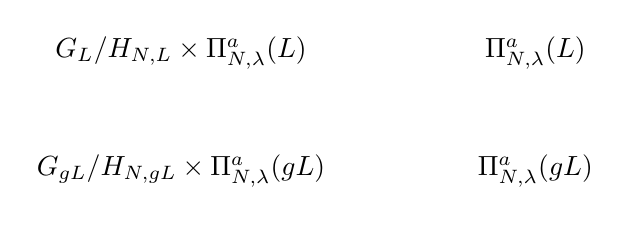
\begin{tikzpicture}[scale=1.5, baseline = -0.5ex]
\node (A) at (0,1) {$G_L/{H_{N,L}}\times\Pi_{N,\lambda}^a(L)$};
\node (B) at (3,1) {$\Pi_{N,\lambda}^a(L)$};
\node (C) at (0,0) {$G_{gL}/{H_{N,gL}}\times\Pi_{N,\lambda}^a(gL)$};
\node (D) at (3,0) {$\Pi_{N,\lambda}^a(gL)$};

\cdarrow (A) edge (B);
\cdarrow (A) edge (C);
\cdarrow (B) edge (D);
\cdarrow (C) edge (D);
\end{tikzpicture}
\end{equation*}

\subsection{Incidence in affine flag varieties}

\begin{lemma}\label{lemma:incidence-varieties-master}
Given $N,a,b,c\in\naturals$, $\lambda,\mu\in\compositions$, $L\in\flags$ and $i,j\in\integers$,
\begin{equation*}
\left\{(L',L'')\in\Pi_{N,\lambda}^a(L)\times\Pi_{N,\mu}^b(L): \dim\left(\frac{L_i'}{L_i'\cap L_j''}\right)\le c\right\}
\end{equation*}
is a closed set in the projective variety $\Pi_{N,\lambda}^a(L)\times\Pi_{N,\mu}^b(L)$.
\end{lemma}

\begin{proof}
There is $M\geq N$ so that $\epsilon^M L_0\subset L_i'\subset\epsilon^{-M}L_0$ and $\epsilon^M L_0\subset L_j''\subset\epsilon^{-M}L_0$. Let $a'=a+(M-N)r$ and $b'=b+(M-N)r$. Lemma \ref{lemma:nesting-subvarieties} shows that $\Pi_{N,\lambda}^a(L)$ is a subvariety of $\Pi_{M,\lambda}^{a'}(L)$, so $\Pi_{N,\lambda}^a(L)\times\Pi_{N,\mu}^b(L)$ is a subvariety of $\Pi_{M,\lambda}^{a'}(L)\times\Pi_{M,\mu}^{b'}(L)$.

The fact that
\begin{equation*}
\dim\left(\frac{L_i'}{L_i'\cap L_j''}\right) = \dim\left(\frac{L_i'/{\epsilon^M L_0}}{L_i'/{\epsilon^M L_0}\cap L_j''/{\epsilon^M L_0}}\right),
\end{equation*}
together with Lemma \ref{lemma:projective-varieties-of-cyclic-flags} and Lemma \ref{lemma:grassmannian-incidence-varieties}, shows that
\begin{equation*}
\left\{(L',L'')\in\Pi_{M,\lambda}^{a'}(L)\times\Pi_{M,\mu}^{b'}(L):\dim\left(\frac{L_i'}{L_i'\cap L_j''}\right)\le c\right\}
\end{equation*}
is closed, so the intersection with $\Pi_{N,\lambda}^a(L)\times\Pi_{N,\mu}^b(L)$ is also closed.
\end{proof}

\begin{lemma}\label{lemma:incidence-varieties-consequences}
Given $N,a,c\in\naturals$, $\lambda\in\compositions$, $L\in\flags$ and $i,j\in\integers$,
\begin{equation*}
\left\{L'\in\Pi_{N,\lambda}^a(L):\dim\left(\frac{L_i}{L_i\cap L_j'}\right)\le c\right\}
\end{equation*}
and
\begin{equation*}
\left\{L'\in\Pi_{N,\lambda}^a(L): \dim\left(\frac{L_j'}{L_i\cap L_j'}\right)\le c\right\}
\end{equation*}
are closed sets in $\Pi_{N,\lambda}^a(L)$.
\end{lemma}

\begin{proof}
This is a result of Lemma \ref{lemma:grassmannian-incidence-lemmas}, since
\begin{equation*}
\dim\left(\frac{L_i'}{L_i'\cap L_j''}\right) = \dim\left(\frac{L_i'/{\epsilon^M L_0}}{L_i'/{\epsilon^M L_0}\cap L_j''/{\epsilon^M L_0}}\right),
\end{equation*}
where $M\geq N$ is chosen so that $\epsilon^M L_0\subset L_i'\subset\epsilon^{-M}L_0$ and $\epsilon^M L_0\subset L_j''\subset\epsilon^{-M}L_0$ for each $(L',L'')\in\Pi_{N,\lambda}^a(L)\times\Pi_{N,\mu}^b(L)$.
\end{proof}


\section{Geometry of orbits}

\begin{lemma}\label{lemma:bounded-orbits}
Given $A\in\matrices$ and $L\in\flags_{\ro{A}}$, there is $N\in\naturals$ such that $\xprod[L]{A}\subset\Pi_{N,\co{A}}^{a}(L)$, where $a=d_{nN,0}{A}$.
\end{lemma}

\begin{proof}
There is $N\in\naturals$ so that $a_{i,j}=0$ whenever $|j-i|>nN$. If $(L,L')\in\orbit{A}$ then
\begin{equation*}
\dim\left(\frac{L_0'}{L_0'\cap\epsilon^{-N}L_0}\right) = \dim\left(\frac{L_0'}{L_0'\cap L_{nN}}\right) = \sum_{s>nN,t\le 0} a_{s,t} = 0,
\end{equation*}
so it follows $L_0'\subset\epsilon^{-N}L_0$. Similarly,
\begin{equation*}
\dim\left(\frac{\epsilon^N L_0}{\epsilon^N L_0\cap L_0'}\right) = \dim\left(\frac{L_{-nN}}{L_{-nN}\cap L_0'}\right) = \sum_{s\le -nN,t>0} a_{s,t} = 0,
\end{equation*}
which shows $\epsilon^N L_0\subset L_0'$. Moreover,
\begin{equation*}
\dim\left(\frac{\epsilon^{-N}L_0}{L_0'}\right) = \dim\left(\frac{\epsilon^{-N}L_0}{\epsilon^{-N}L_0\cap L_0'}\right) = \sum_{s\le nN,t>0}a_{s,t} = d_{nN,0}(A),
\end{equation*}
as a result of Lemma \ref{lemma:codimension-fomula-corner-sums}. 
\end{proof}

\begin{lemma}\label{lemma:orbits-are-quasiprojective}
Given $A\in\matrices$ and $L\in\flags_{\ro{A}}$, $\xprod[L]{A}$ is a locally closed subset of $\Pi_{N,\co{A}}^a(L)$ for some $N\in\naturals$ and where $a=d_{nN,0}{A}$. In particular, $\xprod[L]{A}$ is a quasiprojective variety.
\end{lemma}

\begin{proof}
Lemma \ref{lemma:bounded-orbits} shows that there is $N\in\naturals$ so that $\xprod[L]{A}$ is contained in $\Pi_{N,\lambda}^a(L)$, where $a=d_{nN,0}{A}$ and $\lambda=\co{A}$. If $L'\in\Pi_{N,\lambda}^a(L)$ then
\begin{equation*}
L_{-Nn}=\epsilon^N L_0\subset L_0'\subset L_1'\subset L_n'\subset \epsilon^{-1-N}L_0 = L_{(N+1)n}.
\end{equation*}
Therefore $\xprod[L]{A}$ is the subset of $\Pi_{N,\lambda}^a(L)$ defined by the conditions $\dim(L_i/{L_i\cap L_j'})=d_{i,j}{A}$ for $i:-Nn\le i<j$ and $\dim(L_j'/{L_i\cap L_j'})=\bar{d}_{i,j}{A}$ for $i:j<i\le(N+1)n$, for $j=1,\ldots,n$.

The set of $L'\in\Pi_{N,\lambda}^a(L)$ with $\dim(L_i/{L_i\cap L_j'})\le d_{i,j}{A}$ for $j=1,\ldots,n$ and $i:-Nn\le i<j$ and $\dim(L_j'/{L_i\cap L_j'})\le\bar{d}_{i,j}{A}$ for $j=1,\ldots,n$ and $i:j<i\le(N+1)n$ is a closed subset of $\Pi_{N,\lambda}^a(L)$, as a result of Lemma \ref{lemma:incidence-varieties-consequences}.

On the other hand, the set of $L'\in\Pi_{N,\lambda}^a(L)$ satisfying the conditions $\dim(L_i/{L_i\cap L_j'})\geq d_{i,j}{A}$ (for $i<j$) and $\dim(L_j'/{L_i\cap L_j'})\geq\bar{d}_{i,j}{A}$ (for $i>j$) is open in $\Pi_{N,\lambda}^a(L)$ since the complement is closed, as a result of Lemma \ref{lemma:incidence-varieties-consequences}.

Therefore $\xprod[L]{A}$ is the intersection of an open set and a closed set in $\Pi_{N,\lambda}^a(L)$, so $\xprod[L]{A}$ is locally closed. It follows that $\xprod[L]{A}$ is an open subset of the projective variety $\overline{\xprod[L]{A}}$, so is a quasiprojective variety as claimed. 
\end{proof}

\begin{lemma}\label{lemma:orbits-are-irreducible}
Given $A\in\matrices$ and $L\in\flags_{ro{A}}$, $\xprod[L]{A}$ is irreducible.
\end{lemma}

\begin{proof}
There is $N\in\naturals$ such that $\xprod[L]{A}\subset\Pi_{N,\lambda}^a(L)$, where $\lambda=\co{A}$ and $a=d_{nN,0}{A}$, using Lemma \ref{lemma:bounded-orbits}.

Lemma \ref{lemma:connected-algebraic-group} shows that $G_L/{H_{N,L}}$ is a connected algebraic group acting algebraically on $\Pi_{N,\lambda}^a(L)$, so each orbit is an irreducible locally closed set in $\Pi_{N,\lambda}^a(L)$. In particular, $\xprod[L]{A}$ is irreducible since $\xprod[L]{A} = G_L/{H_{N,L}}\cdot L'$ for any $L'\in\xprod[L]{A}$.
\end{proof}

Consequently, $\overline{\xprod[L]{A}}$ is an irreducible projective variety and the action of $G_L/{H_{N,L}}$ on $\Pi_{N,\lambda}^a(L)$ restricts to an algebraic group action on $\overline{\xprod[L]{A}}$ for which there are finitely many orbits. In particular, $\overline{\xprod[L]{A}}\setminus\xprod[L]{A}$ is a union of finitely many orbits which are so-called degenerations of the orbit $\xprod[L]{A}$.

\subsection{Geometry of orbit products}

Suppose $A,B\in\matrices$ with $\co{A}=\ro{B}$. Recall the notation
\begin{equation*}
\yprod{A,B} = \{(L,L',L'')\in\flags^3: (L,L')\in\orbit{A}, (L',L'')\in\orbit{B}\}
\end{equation*}
and
\begin{equation*}
\xprod{A,B} = \{(L,L'')\in\flags^2:\exists L'\in\flags \text{ with } (L,L',L'')\in \yprod{A,B}\}.
\end{equation*}

$\xprod{A,B}$ is the image of $\yprod{A,B}$ under the forgetful map $(L,L',L'')\mapsto (L,L'')$.

\begin{lemma}\label{lemma:orbit-products-are-bounded}
There is $N\in\naturals$ such that
\begin{equation*}
\epsilon^N L_0\subset L_0''\subset \epsilon^{-N}L_0
\end{equation*}
for each $(L,L'')\in \xprod{A,B}$.
\end{lemma}

\begin{proof}
There exist $N_1,N_2\in\naturals$ such that
\begin{equation*}
\epsilon^{N_1}L_0\subset L_0'\subset \epsilon^{-N_1}L_0
\end{equation*}
and
\begin{equation*}
\epsilon^{N_2}L_0'\subset L_0''\subset \epsilon^{-N_2}L_0',
\end{equation*}
for each $(L,L',L'')\in \yprod{A,B}$. Then, for $(L,L',L'')\in \yprod{A,B}$,
\begin{equation*}
L_0''\subset \epsilon^{-N_2} L_0' \subset \epsilon^{-(N_1+N_2)} L_0
\end{equation*}
and
\begin{equation*}
\epsilon^{N_1+N_2}L_0\subset \epsilon^{N_2}L_0'\subset L_0''.
\end{equation*}

In particular, taking $N=N_1 + N_2$, we have
\begin{equation*}
\epsilon^N L_0 \subset L_0'' \subset \epsilon^{-N}L_0
\end{equation*}
for each $(L,L'')\in \xprod{A,B}$.
\end{proof}

\begin{lemma}\label{lemma:codimensions-in-orbit-product}
Suppose $N_1,N_2\in\naturals$ with $\epsilon^{N_1}L_0\subset L_0\subset \epsilon^{-N_1}L_0$ and $\epsilon^{N_2}L_0'\subset L_0''\subset \epsilon^{-N_2}L_0'$ for each $(L,L',L'')\in \yprod{A,B}$ and let $N = N_1 + N_2$. Then
\begin{equation*}
\dim\left(\frac{\epsilon^{-N}L_0}{L_0''}\right) = d_{nN_1,0}(A) + d_{nN_2,0}(B)
\end{equation*}
and
\begin{equation*}
\dim\left(\frac{L_0''}{\epsilon^N L_0}\right) = 2Nr - d_{nN_1,0}(A) + d_{nN_2,0}(B),
\end{equation*}
for each $(L,L'')\in \xprod{A,B}$.
\end{lemma}

\begin{proof}
Suppose $(L,L'')\in \xprod{A,B}$ and $L'\in\flags$ so that $(L,L',L'')\in \yprod{A,B}$. As in lemma \ref{lemma:orbit-products-are-bounded}, $\epsilon^N L_0\subset L_0''\subset \epsilon^{-N}L_0$, so
\begin{equation*}
\dim\left(\frac{\epsilon^{-N}L_0}{L_0''}\right) + \dim\left(\frac{L_0''}{\epsilon^N L_0}\right) = \dim\left(\frac{\epsilon^{-N}L_0}{\epsilon^N L_0}\right).
\end{equation*}

As a $\field$-vector space, $\epsilon^{-N}L_0/\epsilon^N L_0$ is isomorphic to $(L_0/{\epsilon L_0})^{2N}$, which has dimension $2Nr$, so
\begin{equation*}
\dim\left(\frac{L_0''}{\epsilon^N L_0}\right) = 2Nr - \dim\left(\frac{\epsilon^{-N}L_0}{L_0''}\right).
\end{equation*}

It remains to compute the codimension of $L_0''$ in $\epsilon^{-N}L_0$. Note $L_0''\subset \epsilon^{-N_2}L_0'\subset \epsilon^{-N} L_0$, so
\begin{equation*}
\dim\left(\frac{\epsilon{-N}L_0}{L_0''}\right) = \dim\left(\frac{\epsilon^{-N}L_0}{\epsilon^{-N_2}L_0'}\right) + \dim\left(\frac{\epsilon^{-N_2}L_0'}{L_0''}\right).
\end{equation*}

\begin{align*}
\dim\left(\frac{\epsilon^{-N}L_0}{\epsilon^{-N_2}L_0'}\right)
&= \dim\left(\frac{\epsilon^{-N_1}L_0}{L_0'}\right)\\
&= \dim\left(\frac{L_{nN_1}}{L_{nN_1}\cap L_0'}\right)\\
&= \sum_{s\le nN_1, t>0} A_{s,t}\\
&= d_{nN_1,0}(A).
\end{align*}

\begin{align*}
\dim\left(\frac{\epsilon^{-N_2}L_0'}{L_0''}\right)
&= \dim\left(\frac{ L_{nN_2}'}{L_{nN_2}'\cap L_0''}\right)\\
&= \sum_{s\le nN_2, t>0} B_{s,t}\\
&= d_{nN_2,0}(B).
\end{align*}
\end{proof}

Refer to Section \ref{sec:orbit-product} for definitions of the spaces $\xprod[L]{A,B}$ and $\yprod[L]{A,B}$.

\begin{lemma}
Given $A,B\in\matrices$ with $\ro{B}=\co{A}$ and $(L,L',L'')\in\flags^3$ with $(L,L')\in\orbit{A}$ and $(L',L'')\in\orbit{B}$,
\begin{align*}
\xprod[L]{A,B}
&= G_L G_{L'} L''\\
&= G_L \xprod[L']{B}.
\end{align*}
\end{lemma}

\begin{proof}
$\xprod[L]{A,B}$ is the image of $\yprod[L]{A,B}$ under the forgetful map $(N',N'')\mapsto N''$. If $\alpha\in G_L$ and $\beta\in G_{L'}$ then $(L,\alpha L,\alpha\beta L'')\in\yprod{A,B}$ since $(L,\alpha L')=\alpha(L,L')\in\orbit{A}$ and $(\alpha L',\alpha\beta L'')=\alpha\beta(\beta^{-1}L',L'')=\alpha\beta(L',L'')\in\orbit{B}$. Consequently, $G_L G_{L'}L''\in\xprod[L]{A,B}$.

For the reverse inclusion, if $(N',N'')\in\yprod[L]{A,B}$ then $(L,N')\in\orbit{A}$ and $(N',N'')\in\orbit{B}$, so there exist $\sigma_1,\sigma_2\in G$ such that $(L,N')=\sigma_1(L,L')$ and $(N',N'')\in\sigma_2(N',N'')$. Then $(L,N',N'') = (L,\sigma_1 L',\sigma_1(\sigma_1^{-1}\sigma_2) L'')$ with $\sigma_1\in G_L$ and $\sigma_1^{-1}\sigma_2\in G_{L'}$. Thus $\xprod[L]{A,B} = G_L G_{L'}L''$.

The second equality follows since $\xprod[L']{B}=G_{L'}L''$.
\end{proof}

\begin{lemma}
There is $N\in\naturals$ such that $H_N\subset G_{L'}$. Consequently, $H_{N'}\subset G_{L'}$ whenever $N'\geq N$.
\end{lemma}

\begin{proof}
Choose $N\in\naturals$ such that $\epsilon^N L_0\subset L_0'\subset \epsilon^{-N}L_0$. Then
\begin{equation*}
\epsilon^N L_0 \subset L_0'\subset L_1'\subset\cdots\subset L_n' \subset \epsilon^{-(1+N)}L_0.
\end{equation*}
Let $h\in H_N$. $h(x) + \epsilon^N L_0 = x + \epsilon^N L_0$ for $x\in\epsilon^{-(1+N)} L_0$, so $h(L_i')\subset L_i'$ for $i=0,1,\ldots,n$. Moreover, $h^{-1}$ stabilises $L_i'$, so $h(L_i') = L_i'$ for $i=0,1,\ldots,n$ and therefore for $i\in\integers$. This shows $h\in G_{L'}$ as required, so $H_N\subset G_{L'}$.
\end{proof}

$H_N$ is generally not normal in $G_{L'}$, though the space of (right) cosets of $H_N$ in $G_{L'}$ will still be irreducible.

\begin{lemma}
$G_{L'}/H_N$ is irreducible, provided $H_N\subset G_{L'}$.
\end{lemma}

{\color{blue}
\begin{proof}
Needs a proof.
\end{proof}
}

\begin{lemma}\label{lemma:y-prod-is-quasiprojective}
Given $A,B\in\matrices$ with $\co{A}=\ro{B}$ and $L\in\flags_{\ro{A}}$, $\yprod[L]{A,B}$ is a locally closed set in $\Pi_{N,\lambda}^a(L)\times\Pi_{2N,\mu}^{a+b}(L)$, where $\lambda=\co{A}$, $\mu=\co{B}$, $a=d_{nN,0}{A}$ and $b=d_{nN,0}{B}$. In particular, $\yprod[L]{A,B}$ is a quasiprojective variety.
\end{lemma}

{\color{gray}CONTINUE HERE THURSDAY MORNING}
\begin{proof}
There is $N\in\naturals$ such that $\epsilon^N L_0\subset L_0'\subset\epsilon^{-N}L_0$ and $\epsilon^N L_0'\subset L_0''\subset\epsilon^{-N}L_0'$ for each $(L,L',L'')$ with $(L,L')\in\orbit{A}$ and $(L',L'')\in\orbit{B}$. Let $a=d_{nN,0}(A)$ and $b=d_{nN,0}(B)$. Then $\yprod[L]{A,B}$ is the subset of $\Pi_{N,\co{A}}^a(L)\times\Pi_{2N,\co{B}}^{a+b}(L)$ defined by the conditions
\begin{equation*}
\dim\left(\frac{L_i}{L_i\cap L_j'}\right) = d_{i,j}(A)
\end{equation*}
and
\begin{equation*}
\dim\left(\frac{L_i'}{L_i'\cap L_j''}\right) = d_{i,j}(B)
\end{equation*}
for each $i,j\in\integers$.

{\color{blue} it remains to justify why these are locally closed conditions on the product and why there are effectively only finitely many conditions.}
Thus $\yprod[L]{A,B}$ is a locally closed subset of $\Pi_{N,\co{A}}^a(L)\times\Pi_{2N,\co{B}}^{a+b}(L)$ so is a quasiprojective variety.
\end{proof}

\begin{proposition}\label{prop:irreducible-y-prod}
Given $A,B\in\matrices$ with $\co{A}=\ro{B}$ and $L\in\flags_{\ro{A}}$, $\yprod[L]{A,B}$ is an irreducible quasi-projective variety.
\end{proposition}

\begin{proof}
There is $N\in\naturals$ such that $\epsilon^N L_0\subset L_0'\subset \epsilon^{-N} L_0$ and $\epsilon^N L_0'\subset L_0''\subset\epsilon^{-N}L_0'$ for each $(L',L'')\in\yprod[L]{A,B}$. Write $a=d_{nN,0}(A)$ and $b=d_{nN,0}(B)$, so $\yprod[L]{A,B}\subset\Pi_{N,\co{A}}^a(L)\times\Pi_{2N,\co{B}}^{a+b}(L)$. Lemma \ref{lemma:y-prod-is-quasiprojective} shows that $\yprod[L]{A,B}$ is a locally closed subset of $\Pi_{N,\co{A}}^a(L)\times\Pi_{2N,\co{B}}^{a+b}(L)$ and thus a quasiprojective variety, so it remains to show $\yprod[L]{A,B}$ is irreducible.

For any $L'\in\xprod[L]{A}$, $\yprod[L]{A,B}=G_L\cdot (\{L'\}\times\xprod[L']{B}) = G_L/{H_{2N,L}}\cdot (\{L'\}\times\xprod[L']{B})$. $\overline{\xprod[L']{B}}$ is an irreducible subvariety of $\Pi_{N,\co{B}}^b(L')$, which is a subvariety of $\Pi_{2N,\co{B}}^{a+b}(L)$, so $\{L'\}\times\overline{\xprod[L']{B}}$ is an irreducible subvariety of $\Pi_{N,\co{A}}^a(L)\times\Pi_{2N,\co{B}}^{a+b}(L)$. In particular, $\{L'\}\times\xprod[L']{B}$ is an irreducible (locally closed) subspace of $\Pi_{N,\co{A}}^a(L)\times\Pi_{2N,\co{B}}^{a+b}(L)$. $G_L/{H_{2N,L}}$ is a connected algebraic group acting algebraically on $\Pi_{N,\co{A}}^a(L)\times\Pi_{2N,\co{B}}^{a+b}(L)$ and $\yprod[L]{A,B}$ is the image of $G_L/{H_{2N,L}}\times\{L'\}\times\xprod[L']{B}$ under the action map, so $\yprod[L]{A,B}$ is irreducible. 
\end{proof}

\begin{lemma}\label{lemma:irreducible-x-prod}
Given $A,B\in\matrices$ with $\co{A}=\ro{B}$ and $L\in\flags_{\ro{A}}$, $\xprod[L]{A,B}$ is an irreducible topological space.
\end{lemma}

\begin{proof}
$\xprod[L]{A,B}$ is the image of $\yprod[L]{A,B}$ under the projection $\flags_{\co{A}}\times\flags_{\co{B}}\to\flags_{\co{B}}$ and $\yprod[L]{A,B}$ is irreducible, by Proposition \ref{prop:irreducible-y-prod}, so $\xprod[L]{A,B}$ is irreducible.
\end{proof}

\begin{proof}
There is $N\in\naturals$ such that $\epsilon^N L_0\subset L_0'\subset \epsilon^{-N}L_0$ and $\epsilon^N L_0'\subset L_0''\subset \epsilon^{-N}L_0'$ for each $(L,L')\in\orbit{A}$ and $(L',L'')\in\orbit{B}$. Then $\overline{\xprod[L']{B}}$ is an irreducible subvariety of $\Pi_{N,\co{B}}^b(L')$, which is in turn a subvariety of $\Pi_{2N,\co{B}}^{a+b}(L)$. Thus $\xprod[L']{B}$ is an irreducible subspace of $\Pi_{2N,\co{B}}^{a+b}(L)$. $G_L/{H_{2N,L}}$ is a connected algebraic group acting morphically on $\Pi_{2N,\co{B}}^{a+b}(L)$, therefore $\xprod[L]{A,B} = G_L/{H_{2N,L}}\cdot\xprod[L']{B}$ is irreducible.
\end{proof}

\begin{remark}
$\xprod[L]{A,B}$ is a union of finitely many $G_L$-orbits, each of which is locally closed, so $\xprod[L]{A,B}$ is constructible. Lemma
\ref{lemma:irreducible-x-prod} shows that $\xprod[L]{A,B}$ is irreducible. Investigate whether $\xprod[L]{A,B}$ is actually locally closed and therefore an irreducible quasiprojective variety.
\end{remark}

\begin{proposition}\label{prop:open-orbits-in-product}
Given $A,B\in\matrices$ with $\co{A}=\ro{B}$ and $L\in\flags_{\ro{A}}$, there is a unique open $G_L$-orbit in $\xprod[L]{A,B}$.
\end{proposition}

\begin{proof}
$\xprod[L]{A,B}$ consists of finitely many $G_L$-orbits and is an irreducible topological space, by Lemma \ref{lemma:irreducible-x-prod}. Consequently, $\xprod[L]{C}$ is dense in $\xprod[L]{A,B}$ for some $C\in\matrices_{A,B}$. Lemma \ref{lemma:orbits-are-quasiprojective} shows that $\xprod[L]{C}$ is locally closed in $\xprod[L]{A,B}$, so $\xprod[L]{C}$ is open in $\overline{\xprod[L]{C}}=\xprod[L]{A,B}$. Irreducibility of $\xprod[L]{A,B}$ shows that there is a unique open $G_L$-orbit, since two non-empty open sets in $\xprod[L]{A,B}$ intersect non-trivially, thus any two open $G_L$ orbits in $\xprod[L]{A,B}$ coincide.
\end{proof}

\section{Existence of a maximum}

\begin{lemma}\label{lemma:compare-partial-orders}
Given $A,A'\in\matrices$ with $\ro{A}=\ro{A'}$ and $\co{A}=\co{A'}$, $A'\le A$ if and only if $\xprod[L]{A'}\subset\overline{\xprod[L]{A}}$ for any $L\in\flags_{\ro{A}}$.
\end{lemma}

{\color{blue}
\begin{proof}
Needs a proof.
\end{proof}
}

\begin{proposition}\label{proposition:existence}
Given $A,B\in\matrices$ with $\co{A}=\ro{B}$, $\matrices_{A,B}$ has a maximum element.
\end{proposition}

\begin{proof}
Let $L\in\flags_{\ro{A}}$. $\xprod[L]{A,B}$ is irreducible by Lemma \ref{lemma:irreducible-x-prod} and is the union of finitely many $G_L$-orbits, namely
\begin{equation*}
\xprod[L]{A,B} = \bigcup_{C\in\matrices_{A,B}} \xprod[L]{C}.
\end{equation*}
This shows that $\xprod[L]{C}$ is dense in $\xprod[L]{A,B}$ for some $C\in\matrices_{A,B}$. Lemma \ref{lemma:orbits-are-quasiprojective} shows that the $G_L$-orbits in $\xprod[L]{A,B}$ are locally closed, so a dense $G_L$-orbit is open in $\xprod[L]{A,B}$. Lemma \ref{lemma:compare-partial-orders} shows that the characteristic matrix of the dense $G_L$-orbit is a maximum in $\matrices_{A,B}$.
\end{proof}

\section{Associativity}

Refer to Section \ref{sec:triple-product} for definitions of the spaces $\xprod[L]{A,B,C}$ and $\yprod[L]{A,B,C}$. Recall that $\xprod[L]{A,B,C}$ is the image of $\yprod[L]{A,B,C}$ under the forgetful map $f$, given by $f(L',L'',L''') = L'''$ for each $(L',L'',L''')\in\yprod[L]{A,B,C}$.

\begin{lemma}
Given $A,B,C\in\matrices$ with $\ro{C}=\co{B}$, $\ro{B}=\co{A}$ and a tuple of flags $(L,L',L'',L''')\in\flags^4$ with $(L,L')\in\orbit{A}$, $(L',L'')\in\orbit{B}$ and $(L'',L''')\in\orbit{C}$,
\begin{equation*}
\xprod[L]{A,B,C} = G_L G_{L'} G_{L''} L'''.
\end{equation*}
\end{lemma}

\begin{proof}
Given $\alpha\in G_L$, $\beta\in G_{L'}$ and $\gamma\in G_{L''}$, $(L,\alpha L',\alpha\beta L'',\alpha\beta\gamma L''')\in\yprod{A,B,C}$ since $(L,\alpha L')=\alpha(L,L')\in\orbit{A}$, $(\alpha L',\alpha\beta L'')=\alpha\beta(L',L'')\in\orbit{B}$ and $(\alpha\beta L'',\alpha\beta\gamma L''')=\alpha\beta\gamma(L'',L''')\in\orbit{C}$. This shows $G_L G_{L'} G_{L''}L'''\in\xprod[L]{A,B,C}$.

Given $(N',N'',N''')\in\yprod[L]{A,B,C}$, there exist $\sigma_1,\sigma_2,\sigma_3\in G$ such that $(L,N') = \sigma_1(L,L')$, $(N',N'') = \sigma_2(L',L'')$ and $(N'',N''') = \sigma_3(L'',L''')$; then $N' = \sigma_1 L' = \sigma_2 L'$, $N'' = \sigma_2 L'' = \sigma_3 L''$ and $N''' = \sigma_3 L'''$. Thus
\begin{equation*}
(L,N',N'',N''') = (L,\sigma_1 L', \sigma_1(\sigma_1^{-1}\sigma_2)L'', \sigma_1(\sigma_1^{-1}\sigma_2)(\sigma_2^{-1}\sigma_3)L''')
\end{equation*}
where $\sigma_1\in G_L$, $\sigma_1^{-1}\sigma_2\in G_{L'}$ and $\sigma_2^{-1}\sigma_3\in G_{L''}$.
\end{proof}

\begin{lemma}\label{lemma:y-triple-is-quasiprojective}
Given $A,B,C\in\matrices$ with $\co{A}=\ro{B}$ and $\co{B}=\ro{C}$ and $L\in\flags_{\ro{A}}$, $\yprod[L]{A,B,C}$ is a quasiprojective variety.
\end{lemma}

\begin{proof}
There is $N\in\naturals$ such that $\epsilon^N L_0\subset L_0'\subset \epsilon^{-N}L_0$, $\epsilon^N L_0'\subset L_0''\subset \epsilon^{-N}L_0'$ and $\epsilon^N L_0''\subset L_0'''\subset\epsilon^{-N}L_0''$ for each $(L',L'',L''')\in\yprod[L]{A,B,C}$. Let $a=d_{nN,0}(A)$, $b=d_{nN,0}(B)$ and $c=d_{nN,0}(C)$. Then $\yprod[L]{A,B,C}$ is the subset of $\Pi_{N,\co{A}}^a(L)\times\Pi_{2N,\co{B}}^{a+b}(L)\times\Pi_{3N,\co{C}}^{a+b+c}(L)$ defined by the conditions
\begin{equation*}
\dim\left(\frac{L_i}{L_i\cap L_j'}\right) = d_{i,j}(A),
\end{equation*}
\begin{equation*}
\dim\left(\frac{L_i'}{L_i'\cap L_j''}\right) = d_{i,j}(B),
\end{equation*}
and
\begin{equation*}
\dim\left(\frac{L_i''}{L_i''\cap L_j'''}\right) = d_{i,j}(C)
\end{equation*}
for each $i,j\in\integers$.

{\color{blue} it remains to shows these conditions define locally closed subsets of the triple product and that there are effectively finitely many conditions}.

Thus $\yprod[L]{A,B,C}$ is a locally closed subset of the projective variety $\Pi_{N,\co{A}}^a(L)\times\Pi_{2N,\co{B}}^{a+b}(L)\times\Pi_{3N,\co{C}}^{a+b+c}(L)$, so $\yprod[L]{A,B,C}$ is a quasiprojective variety.
\end{proof}

\begin{lemma}\label{lemma:irreducible-y-triple}
Given $A,B,C\in\matrices$ with $\co{A}=\ro{B}$ and $\co{B}=\ro{C}$ and $L\in\flags_{\ro{A}}$, $\yprod[L]{A,B,C}$ is an irreducible quasiprojective variety.
\end{lemma}

\begin{proof}
There is $N\in\naturals$ such that $\epsilon^N L_0\subset L_0'\subset\epsilon^{-N}L_0$, $\epsilon^N L_0'\subset L_0''\subset\epsilon^{-N}L_0'$ and $\epsilon^N L_0''\subset L_0'''\subset\epsilon^{-N}L_0''$ for each $(L',L'',L''')\in\yprod[L]{A,B,C}$. Lemma \ref{lemma:connected-algebraic-group} shows that $G_L/{H_{3N,L}}$ is a connected algebraic group acting algebraically on $\Pi = \Pi_{N,\co{A}}^a(L)\times\Pi_{2N,\co{B}}^{a+b}(L)\times\Pi_{3N,\co{C}}^{a+b+c}(L)$.

Let $L'\in\xprod[L]{A}$. $\yprod[L]{A,B,C} = G_L\cdot (\{L'\}\times\yprod[L']{B,C}$. $\yprod[L']{B,C}$ is an irreducible quasiprojective variety; $\overline{\yprod[L']{B,C}}$ is an irreducible subvariety of $\Pi_{N,\co{B}}^b(L')\times\Pi_{2N,\co{C}}^{b+c}(L')$, which is a subvariety of $\Pi_{2N,\co{B}}^{a+b}(L)\times\Pi_{3N,\co{C}}^{a+b+c}(L)$. Thus $\{L'\}\times\overline{\yprod[L']{B,C}}$ is an irreducible subvariety of $\Pi$. Therefore $\yprod[L]{A,B,C}$ is the image of the irreducible space $G_L/{H_{3N,L}}\times\{L'\}\times\yprod[L']{B,C}$ under the action map, so $\yprod[L]{A,B,C}$ is irreducible. Lemma \ref{lemma:y-triple-is-quasiprojective} shows that $\yprod[L]{A,B,C}$ is quasiprojective, so $\yprod[L]{A,B,C}$ is an irreducible quasiprojective variety.
\end{proof}

\begin{corollary}\label{lemma:irreducible-x-triple}
Given $A,B,C\in\matrices$ with $\co{A}=\ro{B}$ and $\co{B}=\ro{C}$ and $L\in\flags_{\ro{A}}$, $\xprod[L]{A,B,C}$ is an irreducible topological space.
\end{corollary}

\begin{proof}
$\xprod[L]{A,B,C}$ is the image of $\yprod[L]{A,B,C}$ under the forgetful map $f$ and $\yprod[L]{A,B,C}$ is irreducible, by Lemma \ref{lemma:irreducible-y-triple}, so $\xprod[L]{A,B,C}$ is irreducible.
\end{proof}

\begin{lemma}\label{lemma:generic-triple-product}
Given matrices $A,B,C\in\matrices$ with $\co{A}=\ro{B}$ and $\co{B}=\ro{C}$ and $L\in\flags_{\ro{A}}$, there is a unique open $G_L$-orbit in $\xprod[L]{A,B,C}$.
\end{lemma}

\begin{proof}
$\xprod[L]{A,B,C}$ is irreducible, by Corollary \ref{lemma:irreducible-x-triple}, and consists of finitely many $G_L$-orbits, so contains a dense $G_L$-orbit. In particular, there is $D\in\matrices$ such that $\overline{\xprod[L]{D}}=\xprod[L]{A,B,C}$. Lemma \ref{lemma:orbits-are-quasiprojective} shows that the $G_L$-orbits are locally closed in $\xprod[L]{A,B,C}$. In particular, $\xprod[L]{D}$ is open in $\overline{\xprod[L]{D}} = \xprod[L]{A,B,C}$. Therefore, there is an open $G_L$-orbit in $\xprod[L]{A,B,C}$. There is a unique open $G_L$-orbit since $\xprod[L]{A,B,C}$ is irreducible.
\end{proof}

\begin{lemma}\label{lemma:zprod-open-in-yprod-left}
Given $A,B,C\in\matrices$ with $\co{A}=\ro{B}$ and $\co{B}=\ro{C}$ and $L\in\flags_{\ro{A}}$, $f^{-1}(\xprod[L]{A\ast B,C})$ is open in $\yprod[L]{A,B,C}$.
\end{lemma}

\begin{proof}
\begin{equation*}
f^{-1}(\xprod[L]{A\ast B,C}) = \left\{ (L',L'',L''')\in\yprod[L]{A,B,C}: \dim\left(\frac{L_i}{L_i\cap L_j''}\right) \text{ is maximal, for each }i,j\in\integers \right\}
\end{equation*}
is open in $\yprod[L]{A,B,C}$ since $f^{-1}(\xprod[L]{A\ast B,C})$ is defined by {\color{blue}finitely many} open conditions; the function on $\xprod[L]{A,B}$ given by $L''\mapsto \dim\left(\frac{L_i}{L_i\cap L_j''}\right)$ is lower semicontinuous, so maximising such a function is an open condition in $\xprod[L]{A,B}$.
\end{proof}

\begin{lemma}\label{lemma:zprod-open-in-yprod-right}
Given $A,B,C\in\matrices$ with $\co{A}=\ro{B}$ and $\co{B}=\ro{C}$ and $L\in\flags_{\ro{A}}$, $f^{-1}(\xprod[L]{A,B\ast C})$ is open in $\yprod[L]{A,B,C}$.
\end{lemma}

\begin{proof}
\begin{equation*}
f^{-1}(\xprod[L]{A,B\ast C}) = \left\{ (L',L'',L''')\in\yprod[L]{A,B,C}: \dim\left(\frac{L_i'}{L_i'\cap L_j'''}\right) \text{ is maximal, for each }i,j\in\integers \right\}
\end{equation*}
is open in $\yprod[L]{A,B,C}$, as it is defined by {\color{blue}finitely many} open conditions; the function on $\xprod[L]{A}\times\xprod[L]{A,B\ast C}$ given by $(L',L''')\mapsto\dim\left(\frac{L_i'}{L_i'\cap L_j'''}\right)$ is lower semicontinuous, so maximising this function is an open condition on $\xprod[L]{A}\times\xprod[L]{A,B\ast C}$.
\end{proof}

\begin{conjecture}\label{conjecture:open-embeddings-in-x}
Given $A,B,C\in\matrices$ with $\co{A}=\ro{B}$ and $\co{B}=\ro{C}$ and $L\in\flags_{\ro{A}}$, $\xprod[L]{A\ast B,C}$ and $\xprod[L]{A,B\ast C}$ are open and dense in $\xprod[L]{A,B,C}$.
\end{conjecture}

\begin{remark}
If $f$ is shown to be an open map then this result follows from Lemma \ref{lemma:zprod-open-in-yprod-left} and Lemma \ref{lemma:zprod-open-in-yprod-right}.
\end{remark}

\begin{proposition}\label{proposition:associativity}
Given $A,B,C\in\matrices$ with $\co{A}=\ro{B}$ and $\co{B}=\ro{C}$, $(A\ast B)\ast C = A\ast (B\ast C)$.
\end{proposition}

\begin{proof}
Take $A,B,C\in\matrices$ with $\co{A}=\ro{B}$ and $\co{B}=\ro{C}$ and fix $L\in\flags_{\ro{A}}$.

$\xprod[L]{(A\ast B)\ast C}$ is open in $\xprod[L]{A\ast B,C}$, so $f^{-1}\xprod[L]{(A\ast B)\ast C}$ is open in $f^{-1}\xprod[L]{A\ast B,C}$. Lemma \ref{lemma:zprod-open-in-yprod-left} shows that $f^{-1}\xprod[L]{A\ast B,C}$ is open in $\yprod[L]{A,B,C}$, so $f^{-1}\xprod[L]{(A\ast B)\ast C}$ is open in $\yprod[L]{A,B,C}$. Similarly, $\xprod[L]{A\ast(B\ast C)}$ is open in $\xprod[L]{A,B\ast C}$ and $f^{-1}\xprod[L]{A,B\ast C}$ is open in $\yprod[L]{A,B,C}$, by Lemma \ref{lemma:zprod-open-in-yprod-right}, so $f^{-1}\xprod[L]{A\ast(B\ast C)}$ is open in $\yprod[L]{A,B,C}$.

Lemma \ref{lemma:irreducible-y-triple} shows that $\yprod[L]{A,B,C}$ is irreducible, so $f^{-1}\xprod[L]{(A\ast B)\ast C}$ and $f^{-1}\xprod[L]{A\ast(B\ast C)}$ have nonempty intersection. Therefore the $G_L$-orbits $\xprod[L]{(A\ast B)\ast C}$ and $\xprod[L]{A\ast(B\ast C)}$ intersect nontrivially, so are the same $G_L$-orbit. In particular, $(A\ast B)\ast C= A\ast(B\ast C)$. 
\end{proof}


\section{The generic algebra}

\begin{lemma}\label{lemma:identity-morphisms}
Given $\lambda\in\compositions$ and $A\in\matrices$, $D_\lambda\ast A = A$ if $\ro{A}=\lambda$ and $A\ast D_\lambda = A$ if $\co{A}=\lambda$.
\end{lemma}
\begin{proof}
Lemma \ref{lemma:product-with-diagonal-orbits} shows that $\matrices_{D_\lambda,A} = \{A\}$ if $\lambda=\ro{A}$ and $\matrices_{A,D_\lambda} = \{A\}$ if $\lambda=\co{A}$, which proves the result. 
\end{proof}

\begin{theorem}\label{thm:generic-category}
The following constitutes a small category: the set of objects is $\compositions$ and the set of morphisms is $\matrices$. Given compositions $\lambda,\mu\in\compositions$, the morphisms with source $\lambda$ and target $\mu$ are those matrices $A\in\matrices$ with $\co{A}=\lambda$ and $\ro{A}=\mu$. Given $\lambda,\mu,\nu\in\compositions$ and $A,B\in\matrices$ with $B\colon\lambda\to\mu$ and $A\colon\mu\to\nu$ the composition is $A\ast B\colon\lambda\to\nu$.
\end{theorem}

\begin{proof}
Proposition \ref{proposition:existence} shows that the composition is well defined while Proposition \ref{proposition:associativity} establishes associativity of the composition. Lemma \ref{lemma:identity-morphisms} shows that $D_\lambda\colon\lambda\to\lambda$ is the identity morphism for each $\lambda\in\compositions$. Thus $(\compositions,\matrices,\co,\ro,\ast)$ is a category.
\end{proof}

Write $\gcat$ to denote this so-called `generic category'.

\begin{example}
The objects in $\gcat[2,2]$ are compositions of $2$ into $2$ parts, namely $(0,2)$, $(1,1)$ and $(2,0)$. The set of morphisms from $\lambda$ to $\mu$ is the set of infinite periodic matrices $A\in\matrices[2,2]$ with $\co{A}=\lambda$ and $\ro{A}=\mu$, which is a countably infinite set for any pair of compositions $\lambda,\mu\in\compositions[2,2]$.
\end{example}

\begin{definition}[Generic algebra]\label{def:generic-algebra}
The generic affine algebra $\generic$ is the category $\integers$-algebra of $\gcat$. In particular, $\generic$ is a free $\integers$-module with basis $\{e_A:A\in\matrices\}$ and with associative multiplication given by
\begin{equation*}
e_A\ast e_B = \begin{cases}
e_{A\ast B} &\text{ if } \co{A}=\ro{B}\\
0 			&\text{ if } \co{A}\neq \ro{B}.
\end{cases}
\end{equation*}
The multiplicative identity in $\generic$ is
\begin{equation*}
1 = \sum_{\lambda\in\compositions}e_{D_\lambda}.
\end{equation*}
\end{definition}


\chapter{A realisation of affine zero Schur algebras}

We aim to prove the isomorphism theorem in the cases $r<n$ and $n\le r< 2n$ separately. Below are crude versions of the statements we want to prove.

\begin{theorem}
Assume $r<n$. The map $\psi\colon\generic\to\zeroschur$, given by $\psi(E_i)=E_i$, $\psi(F_i)=F_i$ and $\psi(1_\lambda) = 1_\lambda$, is an isomorphism of $\integers$-algebras.
\end{theorem}

\begin{theorem}
Assume $n\le r< 2n$. There is a unique homomorphism of $\integers$-algebras $\hat{\psi}\colon\generic\to\zeroschur$ such that $\hat{\psi}(R)=R$ and $\hat{\psi}=\psi$ on the subalgebra of $\generic$ generated by the $E_i$, $F_i$ and $1_\lambda$. $\hat{\psi}$ is an isomorphism of $\integers$-algebras.
\end{theorem}

\section{Preliminary results}

Recall from Definition \ref{def:generic-algebra} that the generic algebra $\generic$ is an associative $\integers$-algebra which is a free $\integers$-module with an atomic basis $\{e_A:A\in\matrices\}$: given $A,B\in\matrices$ with $\co{A}=\ro{B}$, $e_Ae_B = e_{A\ast B}$.

\subsection{Elementary basis elements}

Given $i\in[1,n]$ and $\lambda\in\compositions$ such that $\lambda_{i+1}>0$, define
\begin{equation*}
E_{i,\lambda} = e_{D_\lambda + \elem{i}{i+1} - \elem{i+1}{i+1}}
\end{equation*}
and
\begin{equation*}
E_i = \sum_{\lambda\in\compositions:\lambda_{i+1}>0} E_{i,\lambda}.
\end{equation*}

Given $i\in[1,n]$ and $\lambda\in\compositions$ such that $\lambda_i>0$, define
\begin{equation*}
F_{i,\lambda} = e_{D_\lambda + \elem{i+1}{i} - \elem{i}{i}}
\end{equation*}
and
\begin{equation*}
F_i = \sum_{\lambda\in\compositions:\lambda_i>0} F_{i,\lambda}.
\end{equation*}

\subsection{Transpose involution}

\begin{lemma}\label{lemma:transpose-involution-generic}
The $\integers$-module automorphism $\transpose$ of $\generic$ given by $e_A\mapsto e_{A^\transpose}$ is a $\integers$-algebra antihomomorphism: that is,
\begin{equation*}
e_{A^\transpose}\ast e_{B^\transpose} = e_B\ast e_A
\end{equation*}
for each $A,B\in\matrices$. Moreover, $\transpose(E_{i,\lambda}) = F_{i,\lambda+\alpha_i}$, $\transpose(F_{i,\lambda}) = E_{i,\lambda - \alpha_i}$ and $\transpose(1_\lambda) = 1_\lambda$, for permissible $(i,\lambda)\in\integers\times\compositions$.
\end{lemma}
\begin{proof}
This is a consequence of Lemma \ref{lemma:transpose-involution}. {\color{blue}It must also be shown that the transpose operation on $\matrices$ is order preserving.}
\end{proof}

\subsection{Multiplication rules}

\begin{lemma}\label{lemma:multiplication-rule-generic}
Given $A\in\matrices$ and $i\in[1,n]$ such that $\ro{A}_{i+1}>0$,
\begin{equation*}
E_ie_A = e_{A+\elem{i}{p}-\elem{i+1}{p}},
\end{equation*}
where $p=\max\{p'\in\integers: a_{i+1,p'}>0\}$.

Given $A\in\matrices$ and $i\in[1,n]$ such that $\ro{A}_i>0$,
\begin{equation*}
F_ie_A = e_{A+\elem{i+1}{p}-\elem{i}{p}},
\end{equation*}
where $p=\min\{p'\in\integers: a_{i,p'}>0\}$.
\end{lemma}

Similar formulas for right multiplication by $E_i$ and $F_i$ are obtained by applying the transpose.

\section{Presentation of the generic algebra.}

Recall that $\compositions$ denotes the set of compositions of $r$ into $n$ parts. That is, $\compositions$ is the set of tuples $\lambda = (\lambda_1,\ldots,\lambda_n)\in\integers^n$ with each $\lambda_i$ non-negative and $\lambda_1 +\cdots +\lambda_n = r$. Given $i\in [1,n]$, let $\epsilon_i = (0,\ldots,1,\ldots,0)\in\integers^n$ be the $i$--th elementary vector and let $\alpha_i = \epsilon_i - \epsilon_{i+1}$. Then given $\lambda\in\compositions$, we have $\lambda + \alpha_i\in\compositions$ provided $\lambda_{i+1}>0$ and $\lambda - \alpha_i\in\compositions$ provided $\lambda_i>0$.

Let $\Gamma =\presentationquiver$ be the quiver with set of vertices $\compositions$ with arrows $e_{i,\lambda}\colon\lambda\to\lambda +\alpha_i$ (if $\lambda_{i+1}>0$) and $f_{i,\lambda}\colon\lambda\to\lambda -\alpha_i$ (if $\lambda_i>0$). Thus there are no arrows between $\lambda$ and $\mu$ unless $\lambda = \mu\pm \alpha_i$ for some $i\in [1,n]$.

If $n\geq 3$ then neighbouring vertices are connected by two arrows, one of each direction. In the case $n=2$, neighbouring vertices are joined by four arrows, two of each direction. The $\integers\Gamma$ denote the path $\integers$ algebra of $\Gamma$. By construction of $\Gamma$, there is a $\integers$-algebra homomorphism $\integers\Gamma\to\generic$ with $e_{i,\lambda}\mapsto E_{i,\lambda}$, $f_{i,\lambda}\mapsto F_{i,\lambda}$ and $k_\lambda = 1_\lambda$. We aim to describe the image and kernel of the morphism to give a presentation of the generic algebra by a quiver with relations, when possible. In general, we should obtain a presentation of a subalgebra of the generic algebra consisting of the so-called aperiodic elements (c.f. \cite{lusztig99}).

\begin{definition}(aperiodicity)\label{def:aperiodic}
$A\in\matrices$ is aperiodic if for each $l\in\integers\setminus\{0\}$ there exists $i\in\integers$ such that $a_{i,i+l}=0$. Denote the set of aperiodic elements in $\matrices$ by $\matrices^{ap}$. Note that $\matrices^{ap}=\matrices$ if $r<n$. Linear combinations of the basis elements corresponding to aperiodic matrices are also said to be aperiodic - if $A$ is aperiodic, we say $e_A$ is aperiodic.
\end{definition}

\begin{lemma}\label{lemma:words-are-aperiodic}
Let $A\in\matrices$ and write $\lambda=\ro{A}$. If $A$ is aperiodic and $\lambda_{i+1}>0$, then $E_i\ast e_A$ is aperiodic. If $A$ is aperiodic and $\lambda_i>0$, then $F_i\ast e_A$ is aperiodic.
\end{lemma}

\begin{proof}
Suppose $A\in\matrices$ is aperiodic and $\lambda_{i+1}>0$, where $\lambda=\ro{A}$. There is $p\in\integers$ such that $a_{i+1,p}>0$ and $a_{i+1,p'}=0$ whenever $p'>p$. Lemma \ref{lemma:multiplication-rule-generic} shows that $E_i\ast e_A = e_B$, where $B=A+\elem{i}{p}-\elem{i+1}{p}$. Let $l\in\integers\setminus\{0\}$. If $l\notin\{p-i,p-i-1\}$, then $b_{s,s+l}=a_{s,s+l}$ for each $s\in\integers$, so there is $s\in\integers$ such that $b_{s,s+l}=a_{s,s+l}=0$, since $A$ is aperiodic. If $l=p-i$, then $b_{i+1,i+1+l} = b_{i+1,p+1}=a_{i+1,p+1}=0$, by maximality of $p$. If $l=p-i-1$, there is $s\neq i+1$ such that $a_{s,s+l}=0$, since $A$ is aperiodic and $a_{i+1,i+1+l}=a_{i+1,p}>0$, so $b_{s,s+l}=a_{s,s+l}=0$. Therefore, $B=A+\elem{i}{p}-\elem{i+1}{p}$ is aperiodic.

Suppose $A\in\matrices$ is aperiodic and $\lambda_i>0$, where $\lambda=\ro{A}$. Lemma \ref{lemma:multiplication-rule-generic} shows that $F_i\ast e_A = e_C$ where $C=A+\elem{i+1}{p}-\elem{i}{p}$ and $p=\min\{p'\in\integers: a_{i,p'}>0\}$. Let $l\in\integers\setminus\{0\}$. If $l\notin\{p-i,p-i-1\}$ then $c_{s,s+l}=a_{s,s+l}$ for each $s\in\integers$, so there is $s\in\integers$ such that $c_{s,s+p}=a_{s,s+p}=0$, by aperiodicity of $A$. If $l=p-i$, then $a_{i,i+l}=a_{i,p}>0$, so there is $s\neq i$ such that $a_{s,s+l}=0$. Then $c_{s,s+l}=a_{s,s+l}=0$. Finally, if $l=p-i-1$, then $c_{i,i+l}=a_{i,p-1}=0$ by minimality of $p$. Thus $C$ is aperiodic as required.
\end{proof}

\begin{definition}(Weight function)\label{def:weight-function}
Define the weight function $\weight\colon\matrices\to\integers$ by
\begin{equation*}
\weight{A} = \sum_{i\in[1,n],j\in\integers} |j-i|a_{i,j}
\end{equation*}
for each $A\in\matrices$. The sum is taken over a transversal of the set of congruence classes of $(i,j)$ modulo $(n,n)$ for $i,j\in\integers$.
\end{definition}

\begin{lemma}\label{lemma:decreasing-weight}
Let $A\in\matrices$ and write $\lambda=\ro{A}$. Suppose $\lambda_{i+1}>0$ and set $p=\max\{p'\in\integers: a_{i+1,p'}>0\}$. If $p>i$ then $\weight{e_{i,\lambda}\ast A}=1+\weight{A}$. If $p\le i$ then $\weight{e_{i,\lambda}\ast A}=-1+\weight{A}$. Suppose $\lambda_i>0$ and set $q=\min\{q'\in\integers: a_{i,q'}>0\}$. If $q\le i$ then $\weight{f_{i,\lambda}\ast A}=1+\weight{A}$. If $q>i$ then $\weight{f_{i,\lambda}\ast A}=-1+\weight{A}$.
\end{lemma}

\begin{proof}
Lemma \ref{lemma:multiplication-rule-generic} shows that $e_iA = A+\elem{i}{p}-\elem{i+1}{p}$, so $\weight{e_iA} - \weight{A} = |p-i| - |p-i-1|$, which equals $1$ if $p>i$ and equals $-1$ if $p\le i$. Similarly, $f_iA = A + \elem{i+1}{q} - \elem{i}{q}$ by Lemma \ref{lemma:multiplication-rule-generic}, so $\weight{f_iA} - \weight{A} = |q-i-1| - |q-i|$, which equals $-1$ if $q>i$ and equals $1$ if $q\le i$.
\end{proof}

\begin{lemma}\label{lemma:factorising-aperiodic-elements}
If $A\in\matrices$ is aperiodic, then $e_A$ may be obtained from $1_{\co{A}}$ by finitely many applications of $E_i$ and $F_i$ for $i\in[1,n]$.
\end{lemma}

\begin{proposition}
The $\integers$-subalgebra of $\generic$ generated by $E_{i,\lambda}$, $F_{i,\lambda}$ and $1_\lambda$ has $\integers$-basis $\{e_A:A\in\matrices^{ap}\}$, where $\matrices^{ap}\subset\matrices$ is the set of aperiodic elements.
\end{proposition}

\begin{proof}

\end{proof}

\subsection{The typical case.}

\begin{lemma}
The following relations hold in $\generic$ ($n\geq 3$):
\begin{equation*}
E_iE_j - E_jE_i = 0
\end{equation*}
\begin{equation*}
F_iF_j - F_jF_i = 0
\end{equation*}
unless $|j-i|=1$.
\begin{equation*}
E_iE_{i+1}^2 - E_{i+1}E_iE_{i+1} = 0
\end{equation*}
\begin{equation*}
E_i^2E_{i+1} - E_iE_{i+1}E_i = 0
\end{equation*}
\begin{equation*}
F_{i+1}F_i^2 - F_iF_{i+1}F_i = 0
\end{equation*}
\begin{equation*}
F_{i+1}^2F_i - F_{i+1}F_iF_{i+1} = 0
\end{equation*}

\begin{equation*}
E_iF_j - F_jE_i = 0
\end{equation*}
unless $j=i$.
\begin{equation*}
E_iFi - F_iE_i + \sum_{\lambda:\lambda_i = 0,\lambda_{i+1}>0} 1_\lambda - \sum_{\lambda:\lambda_i>0, \lambda_{i+1}=0} 1_\lambda = 0.
\end{equation*}
\end{lemma}

\subsection{Exceptional case.}

In this case, the quiver $\presentationquiver[2,r]$ has vertices $\compositions[2,r]=\{(0,r), (1,r-1),\ldots, (r,0)\}$; adjacent vertices are connected by two pairs of arrows with opposite orientation: $(e_1,f_1)$ and $(e_2,f_2)$. The relations arising from $\generic[2,r]$ are of a more complicated form - in particular, the serre relations of total degree $3$ will not hold in this case - so this case will be treated separately and at a later date.

\chapter{Further directions}

\section{Further results on affine zero Schur algebras}

[1] Investigate link between this generic product and the generic extension of representations. Shifting to the non-negative subalgebra to do computations purely in terms of generic extensions of quiver representations.

\section{Deformed group algebras of symmetric groups}

[2] Degenerate group algebras of symmetric groups: write down a presentation of the degenerate group algebras, with generators given by the transpositions, or $2$-cycles. Type up the computations done for degenerate group algebras for $S_3$ and $S_4$. Formulate propositions for the general case: the transpositions generate the degenerate group algebra; lemma: `these' relations hold; these generators and relations give a presentation of the degenerate group algebras.

Terminology: deformed group algebra.

% --- END OF DOCUMENT BODY --- %

\printbibliography

\end{document}
